 \documentclass[11pt, a4paper]{article}
\usepackage[utf8]{inputenc}
\usepackage[spanish]{babel}	%Idioma

%Añadir imágenes
\usepackage{graphicx} 	
\usepackage{caption}
\usepackage{subcaption}

%Añadir figuras
\usepackage{float}

%Ajustar márgenes
\usepackage{geometry}	

%Listas
\usepackage{listings}
\usepackage{enumerate}
\usepackage{enumitem}

%Hipervínculos y referencias cruzadas
\usepackage[hidelinks]{hyperref} 

%Opciones de fuente:
\usepackage[default]{sourcesanspro}
\usepackage{sourcecodepro}
\usepackage[T1]{fontenc}

\setlength{\parindent}{15pt}
\setlength{\headheight}{15pt}
\setlength{\voffset}{10mm}

%Opciones de encabezado y pie de página:
\usepackage{fancyhdr}
\pagestyle{fancy}
\renewcommand{\sectionmark}[1]{\markright{#1}{}}
\lhead{\nouppercase\rightmark}
\rhead{Trabajo Fin de Grado}
\lfoot{Grado en Ingeniería Informática}
\cfoot{}
\rfoot{\thepage}
\renewcommand{\headrulewidth}{0.4pt}
\renewcommand{\footrulewidth}{0.4pt}

% Custom colors
\usepackage{xcolor}
\hypersetup{
    colorlinks=true,
    linkcolor=black,
    urlcolor=blue,
    citecolor=blue
}

%Subrayar párrafos

\definecolor{shadecolor}{HTML}{ddf6dd}
\newcommand{\mybox}[1]{\par\noindent\colorbox{shadecolor}
{\parbox{\dimexpr\textwidth-2\fboxsep\relax}{#1}}}

% Eliminar nombre del apartado referencias
\usepackage{etoolbox}
\patchcmd{\thebibliography}{\section*{\refname}}{}{}{}

% Paquete para crear el glosario.
\usepackage[style=super,nonumberlist,toc, acronym, 
    section=section,numberedsection=false
    ]{glossaries}

\makeglossaries

\loadglsentries{glosario.tex}

% Paquete para añadir citas literales
\usepackage{dirtytalk}

% Títulos de párrafos personalizados

\usepackage{titlesec}
\setcounter{secnumdepth}{4}
\setcounter{tocdepth}{4}

\titleformat{\paragraph}
{\normalfont\normalsize\bfseries}{\theparagraph}{1em}{}
\titlespacing*{\paragraph}
{0pt}{3.25ex plus 1ex minus .2ex}{1.5ex plus .2ex}

%Nombre de las tablas
\renewcommand\spanishtablename{Tabla}

%Notas al pie de página
%\renewcommand*\footnoterule{}

\begin{document}
    \sloppy
    
    % Portada
    \begin{titlepage}
    \centering
    
    \vspace*{-2cm}  
    
\includegraphics[width=0.6\textwidth]{portada/logo.png}\par
    
    \vspace{0.5cm}
    \Large{TRABAJO FIN DE GRADO\par}\par
    
    \vspace{0.4cm}
    \large {GRADO EN INGENIERÍA INFORMÁTICA}\par
    
    \vspace{1.5cm}
    \huge{
        \bfseries{Reimplementación de videojuegos clásicos en Three.js utilizando técnicas de generación procedimental}
    }\par
    
    \vspace{1.5cm}
    \large{
        \textbf{Autor} \\ Guillermo Sandoval Schmidt\par
        \vspace{0.5cm}
        \textbf{Director} \\ Francisco Velasco Anguita\par
    }
    
    \vfill
    {\large Granada, noviembre de 2021 \par}
\end{titlepage}
    
    % Prefacio
    \input{prefacio/español}
	
\newpage

\thispagestyle{empty}

\begin{center}
	{\Large\bfseries Re-implementation of classic videogames in Three.js using procedural generation techniques}\\
\end{center}

\begin{center}
	Guillermo Sandoval Schmidt\\
\end{center}

\vspace{0.5cm}
\noindent{\textbf{Keywords:} \textit{procedural content generation}, \textit{Pac-Man}, \textit{maze generation}, \textit{texture generation}, \textit{taxonomy}, \textit{procedural generation in videogames}, \textit{Three.js}, \textit{classic videogames}, \textit{Voronoi Tessellation}.}

\vspace{0.7cm}
\noindent{\textbf{Abstract:}}\\

In 1980 \textit{Rogue} was published, the father of \textit{rogue-like} games and the forerunner of what we know today as procedural content generation.  These techniques have been applied in many fields but especially in the video game industry.  In order to learn about procedural generation, we will make an introduction to it by first understanding what it is and where it is used, and then we will go into the taxonomies proposed to classify both the content and the methods used to generate it. We will also look at the desirable properties of these algorithms and see how they have been used over the years in the video game industry.\\

On the other hand, this project aims to re-implement the classic video game \textit{Pac-Man} by applying procedural generation to the creation of mazes, generating both the layout of the mazes and the textures of the walls.  For the generation of the maze, an algorithm based on pseudo-random number generators and \textit{Tetris}-style pieces has been implemented to compose the maze. For the textures, a shader based on \textit{Voronoi Tessellation} has been implemented.  This was coupled with the challenge of using a graphics library called \textit{Three.js} instead of a game engine.\\

The project has been successful as the generated mazes meet almost all the desirable properties for procedural content generation methods, generating a wide range of valid and playable mazes quickly that could have been designed by a person.

\newpage

\thispagestyle{empty}

\noindent\rule[-1ex]{\textwidth}{1pt}\\[4.5ex]

Yo, \textbf{Guillermo Sandoval Schmidt}, estudiante del Grado en Ingeniería Informática de la Escuela Técnica Superior de Ingenierías Informática y de Telecomunicación de la Universidad de Granada, con DNI
77138466-P,

\vspace{0.5cm}

\textbf{Autorizo:}

\vspace{0.5cm}

La ubicación de la siguiente copia de mi Trabajo Fin de Grado en la biblioteca del centro para que pueda ser consultada por las personas que lo deseen.

\vspace{0.5cm}

Y para que conste, firmo la presente autorización en Granada a \today.

\newpage

\thispagestyle{empty}

\noindent\rule[-1ex]{\textwidth}{1pt}\\[4.5ex]

Yo, \textbf{Guillermo Sandoval Schmidt}, estudiante del Grado en Ingeniería Informática de la Escuela Técnica Superior de Ingenierías Informática y de Telecomunicación de la Universidad de Granada, con DNI
77138466-P,

\vspace{0.5cm}

\textbf{Asumo:}

\vspace{0.5cm}

La originalidad del trabajo, entendida en el sentido de que no se han utilizado fuentes sin citarlas debidamente.

\vspace{0.5cm}

Y para que conste, firmo la presente autorización en Granada a \today.

\newpage

\thispagestyle{empty}

\noindent\rule[-1ex]{\textwidth}{1pt}\\[4.5ex]

Yo, D. \textbf{Francisco Velasco Anguita}, Profesor del Departamento de Lenguajes y Sistemas Informáticos de la Universidad de Granada,

\vspace{0.5cm}

\textbf{Informo:}

\vspace{0.5cm}

Que el presente trabajo, titulado \textit{\textbf{Reimplementación de videojuegos clásicos en Three.js utilizando técnicas de generación procedimental}},
ha sido realizado bajo mi supervisión por D. \textbf{Guillermo Sandoval Schmidt}, y autorizo la defensa de dicho trabajo ante el tribunal
que corresponda.

\vspace{0.5cm}

Y para que conste, expido y firmo el presente informe en Granada a 17 de noviembre de 2021.
    
    \setcounter{page}{6} % Establece el contador para ajustarse al número de páginas del PDF (6 es el número de página del índice menos 1)
    
    % Índice
    \newpage
    \tableofcontents
    
    % Índice de figuras
    \newpage
    \addcontentsline{toc}{section}{\listfigurename}
    \listoffigures
    
    % Índice de tablas
    \newpage
    \renewcommand{\listtablename}{Índice de tablas}
    \addcontentsline{toc}{section}{\listtablename}
    \listoftables
    
    % Introducción 
    \newpage
    \section{Introducción}

Este proyecto se centra en la investigación y aprendizaje sobre generación procedimental de contenidos (\acrshort{pcg} por su sigla en inglés, \acrlong{pcg}), con el fin de estudiar la viabilidad de aplicación de dicha técnica a la reimplementación de videojuegos clásicos. Además, se ha planteado como objetivo la utilización de diversos métodos de \acrshort{pcg} en la implementación de uno de estos videojuegos.\\

Junto con este objetivo principal, dicha implementación se afrontará sin recurrir a un motor de videojuegos, como podría ser Unity, Unreal Engine o Godot, y usando exclusivamente la biblioteca de alto nivel para gráficos \acrshort{3d} en JavaScript, Three.js \cite{three.js}.\\

Durante el desarrollo de este proyecto se requerirá aplicar los conocimientos adquiridos en el Grado en Ingeniería Informática, haciendo especial mención a las asignaturas \textit{``Informática Gráfica''} y \textit{``Sistemas Gráficos''} ya que abarcan el grueso del desarrollo del videojuego.\\

A continuación se muestra la motivación y objetivos del trabajo, continuando con una sección con la planificación realizada, una descripción de los recursos a utilizar, la metodología que se seguirá y la viabilidad del proyecto. Seguiremos con una sección en la que definiremos la generación procedimental de contenidos y haremos un recorrido histórico por su uso en los videojuegos, clasificando el contenido generado, los métodos empleado para generarlo y estableceremos una serie de propiedades deseables asociadas a la generación procedimental de contenido. A continuación, analizaremos el juego clásico escogido y haremos una propuesta de elementos a los que aplicar generación procedimental. Seguiremos con una breve sección de diseño que incluye diagramas de clase y modelos jerárquicos. Más adelante entraremos de lleno en la implementación de juego, haciendo breves menciones a los apartados más generales de funcionamiento del propio juego y centrándonos en la generación procedimental de contenido. Finalmente encontramos una sección que incluye las conclusiones alcanzadas con este trabajo y posibles trabajos futuros fruto del proyecto realizado. Además se incluye una sección con las referencias utilizadas y dos anexos, uno que incluye un manual de usuario y otro con un pequeño glosario.

% ---------------------------------------------------------------------------- %

\subsection{Motivación}

Este proyecto está motivado por el interés por aprender sobre la generación procedimental de contenido aplicada a videojuegos combinado con la afición y admiración por los videojuegos clásicos originarios de las máquinas arcade de los años 80. Por ello se ha propuesto un proyecto que combina ambos intereses, con el fin de aplicar técnicas de \acrshort{pcg} a videojuegos que originalmente no plantearon el uso de las mismas.\\

Además, con el fin de mejorar el aprendizaje sobre desarrollo de videojuegos a más bajo nivel, se ha planteado el uso de una biblioteca gráfica, concretamente Three.js \cite{three.js}, frente a un motor de videojuegos como Unity \cite{unity}.

% ---------------------------------------------------------------------------- %

\subsection{Objetivos}

Con las bases del proyecto establecidas, se plantea como objetivo general:

\begin{itemize}
    \item La investigación y el autoaprendizaje sobre generación procedimental de contenidos.
\end{itemize}

Por otro lado, se desarrollaran los siguientes objetivos específicos:

\begin{itemize}
    \item La aplicación de generación procedimental de contenidos a videojuegos clásicos, aplicando diversas técnicas.
    \item La reimplementación del videojuego clásico Pac-Man utilizando técnicas de bajo nivel y sin la ayuda de un motor de videojuegos.
\end{itemize}

% ---------------------------------------------------------------------------- %
    
    % Planificación
    \newpage
    \section{Planificación}

En este apartado haremos un breve recorrido por los recursos que utilizaremos a nivel software y hardware, ya que a nivel de recursos humanos es un proyecto de un solo estudiante (con la supervisión del tutor); mediante diagramas de Gantt veremos la planificación temporal del proyecto; hablaremos de la metodología de desarrollo escogida; y finalmente comentaremos la viabilidad del proyecto.

% ---------------------------------------------------------------------------- %

\subsection{Recursos}

\subsubsection{Hardware}
    
    \textbf{Equipo principal:} Equipo personal a medida
    \begin{itemize}
        \item \textbf{CPU:} Intel(R) Core(TM) i5-10500H 2.90GHz. 6 sockets con 2 núcleos/socket.
        \item \textbf{GPU:} Gigabyte GeForce RTX 3060 Ti EAGLE OC
        \item \textbf{RAM:} 16 GB
    \end{itemize}
    
    \textbf{Equipo secundario:} Lenovo IdeaPad 330
    \begin{itemize}
        \item \textbf{CPU:} Intel(R) Core(TM) i5-8300H 2.30GHz. 2 sockets con 4 núcleos/socket.
        \item \textbf{GPU:} NVIDIA GeForce RTX 1050
        \item \textbf{RAM:} 8 GB
    \end{itemize}

\subsubsection{Software}

\paragraph{Biblioteca gráfica: Three.js}

    Aunque habitualmente el uso de un lenguaje o una biblioteca específica no es más que un tema menor en el desarrollo de un proyecto, en este caso sí es un elemento a tener en cuenta, ya que al no usar un motor de juegos, se aporta un elemento de complejidad y un valor añadido al trabajo.\\
    
    Con ese fin se ha escogido la biblioteca de alto nivel para gráficos 3D en JavaScript, Three.js, que nos permite crear gráficos y animaciones 3D en un navegador web. Además es una biblioteca libre y disponible en GitHub \cite{githubThree}.\\
    
    El uso de esta herramienta frente a un motor de juegos clásico supondrá que todo lo relacionado con físicas, colisiones, controles, etc. quedará bajo nuestra responsabilidad, mientras que nos facilitará el tratamiento de gráficos y nos dará una mayor flexibilidad a la hora de desarrollar el proyecto.

\paragraph{Control de versiones: Git y GitHub}

    De cara a llevar un control de versiones y facilitar el seguimiento del desarrollo del proyecto, se ha decidido usar el software libre Git \cite{git}. El uso de esta herramienta facilitará seguir una metodología incremental a la hora del desarrollo, metodología de la que hablaremos más adelante.\\
    
    De manera complementaria a Git se utilizará la forja Github \cite{github} como plataforma de desarrollo colaborativa, ya que sirve para alojar proyectos que utilicen el control de versiones que nos ofrece Git. Aunque el proyecto a nivel de recursos humanos solo sea llevado por una persona, el uso de una plataforma colaborativa facilita el uso de dos equipos, el seguimiento del proyecto por parte del tutor y abre la posibilidad de compartir el proyecto e incluso desplegarlo con Github Pages \cite{githubPages}.

\subsection{Desarrollo}

\subsubsection{Diagrama de Gantt}

    Como parte de la planificación, se ha realizado un cronograma del proyecto mediante un diagrama de Gantt. El diagrama nos permitirá llevar un control del tiempo previsto para cada apartado del proyecto y realizar modificaciones en la planificación si es necesario. Inicialmente, se propone una planificación con una duración de 30 semanas.\\
    
    Entrando ya en la planificación propuesta, se ha divido la planificación del proyecto en los siguientes tres bloques principales:
    
    \begin{itemize}
        \item \textbf{Investigación:} refleja el tiempo previsto a emplear en el análisis del funcionamiento del juego como la propia investigación y autoaprendizaje sobre generación procedimental y cómo poder aplicarla a nuestro juego.
        \item \textbf{Desarrollo:} refleja el tiempo previsto a emplear en el desarrollo e implementación de la aplicación. Dividiremos la cronología en el juego en sí y los apartados relacionados con \acrshort{pcg}, previsiblemente siendo generación de escenarios, texturas e modificación de la dificultad y/o el comportamiento de la inteligencia artificial.
        \item \textbf{Documentación:} refleja el tiempo previsto a emplear la realización de la memoria del proyecto y de la inclusión de bibliografía en el mismo, por lo que en muchas ocasiones, se realizará en paralelo junto al apartado de investigación.
    \end{itemize}
    
    Mencionar que las semanas 8 y 9 se han dejado en blanco debido a que coinciden con el periodo de exámenes. También aclarar que aunque se incluye la semana 30, ha sido únicamente por una cuestión estética en la presentación del diagrama, ya esa semana forma parte de la entrega del proyecto.

    \begin{figure}[H]
    \begin{center}
        \begin{subfigure}[b]{0.95\textwidth}
            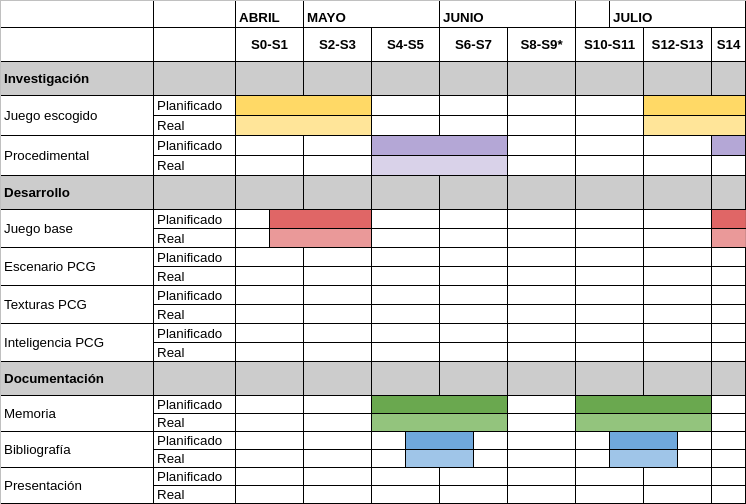
\includegraphics[width=\textwidth]{img/gantt-A.PNG}
            \caption{Planificación desde abril hasta julio.}
        \end{subfigure}
        \par\bigskip
        \begin{subfigure}[b]{0.95\textwidth}
            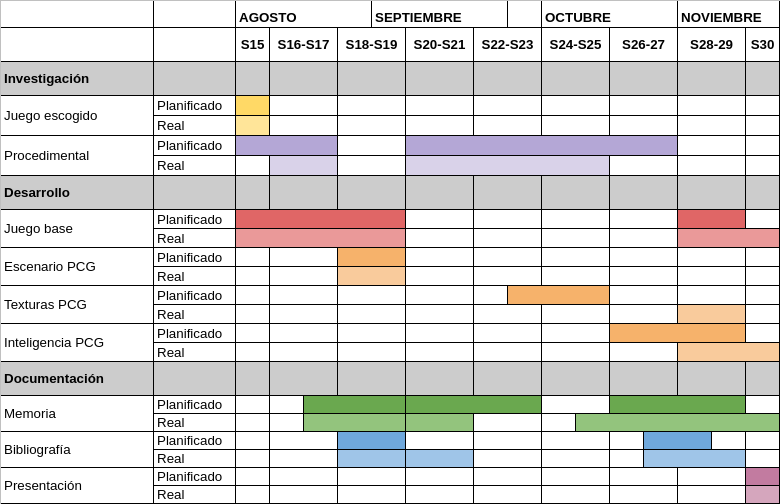
\includegraphics[width=\textwidth]{img/gantt-B.PNG}
            \caption{Planificación desde agosto hasta noviembre.}
        \end{subfigure}
        \caption{Diagrama de Gantt con el tiempo planificado y real para cada hito del proyecto.}
    \end{center}
\end{figure}
    
    
    \begin{table}[H]
        \centering
        \caption{Leyenda del diagrama de Gantt.}
        \begin{tabular}{|l|l|l|l|l|l|}
        \hline
        S0 & 19-25 abril       & S10 & 28 junio - 4 julio       & S20 & 6-12 septiembre         \\ \hline
        S1 & 26 abril - 2 mayo & S11 & 5-11 julio               & S21 & 13-19 septiembre        \\ \hline
        S2 & 3 - 9 mayo        & S12 & 12-18 julio              & S22 & 20-26 septiembre        \\ \hline
        S3 & 10 - 16 mayo      & S13 & 19-25 julio              & S23 & 27 septiembre-3 octubre \\ \hline
        S4 & 17-23 mayo        & S14 & 26 julio - 1 agosto      & S24 & 4-10 octubre            \\ \hline
        S5 & 24-30 mayo        & S15 & 2-8 agosto               & S25 & 11-17 octubre           \\ \hline
        S6 & 31 mayo - 6 junio & S16 & 9-15 agosto              & S26 & 18-24 octubre           \\ \hline
        S7 & 7-13 junio        & S17 & 16-22 agosto             & S27 & 25-31 octubre           \\ \hline
        S8 & 14-20 junio       & S18 & 23-29 agosto             & S28 & 1-7 noviembre           \\ \hline
        S9 & 21-27 junio       & S19 & 30 agosto - 5 septiembre & S29 & 8-14 noviembre          \\ \hline
        \end{tabular}
    \end{table}

\subsubsection{Metodología}

    De cara al modelo de trabajo, siendo un proyecto desarrollado por una sola persona, se plantea llevar una metodología incremental en la que se irán desarrollando, implementando y testeando las distintas funcionalidades que deba tener el juego escogido.\\
    
    Para ello y tal como puede ver en los diagramas de Gantt, se propone dividir el desarrollo en dos hitos con un peso similar, el juego base y la generación procedimental de contenidos, dividiéndose cada uno de ellos en distintas funcionalidades.\\
    
    Esta metodología nos permitirá ir desarrollando el proyecto en paralelo a la investigación sobre la \acrshort{pcg}, obteniendo a lo largo del mismo versiones funcionales del juego con las que realizar pruebas y mejoras durante todo el desarrollo.

\subsection{Viabilidad}

    A la vista de los recursos disponibles, siendo más que suficientes tanto en el apartado hardware como software; contando con un plazo de tiempo bien planificado y una planificación que permite modificaciones en caso de ser necesario; y siguiendo una metodología sencilla pero eficaz que facilita un desarrollo constante del proyecto a la vez que nos permite introducir cambios con facilidad en la aplicación; podemos concluir que el proyecto es viable en la forma y plazos planteados.
    
    % Estado del arte
    \newpage
    \section{Estado del arte}

En este apartado daremos un definición general sobre qué es la generación procedimental de contenidos, dónde y para qué se usa; haremos un recorrido histórico desde los precursores de la \acrshort{pcg} hasta la actualidad; y finalmente entraremos a tratar con más detalle la \acrshort{pcg} en los videojuegos, estableciendo una clasificación del contenido generado y de los métodos más utilizados en \acrshort{pcg}.

\subsection{Generación procedimental de contenidos (PCG)}

\subsubsection{¿Qué es la PCG?}

Antes de comenzar, debemos describir qué es la \acrshort{pcg}. En nuestro caso partiremos de la definición dada en 2015 por Gillian Smith, en el que define la \acrshort{pcg} como: \\

\say{\textit{El uso de un algoritmo formal para generar contenido [...] que normalmente sería producido por un humano}}\cite{smith2015}.\\

Debido al uso de algoritmos, es un error frecuente su asociación con los videojuegos, la animación y los ordenadores en general. Aunque es cierto que sus usos más comunes son la creación de modelados y texturas o la automatización de la generación de grandes cantidades de contenido en un juego, la \acrshort{pcg} se ha usado y se usa en otros campos como la música que veremos a continuación.\\

Si lo orientamos al ámbito de los juegos, es interesante como Smith \cite{smith2015} no establece la \acrshort{pcg} como un problema que se podría enmarcar únicamente en el ámbito de la inteligencia artificial (\acrshort{ai} por su sigla en inglés, \acrlong{ai}), cuyo objetivo sería el de reemplazar o imitar el contenido generado por un diseñador humano, sino que lo establece como un problema más amplio que se superpone con el diseño de juegos, pudiendo ser aplicada la \acrshort{pcg} tanto por ordenadores como por humanos.\\

\begin{figure}[H]
    \begin{center}
        \begin{subfigure}[b]{0.24\textwidth}
            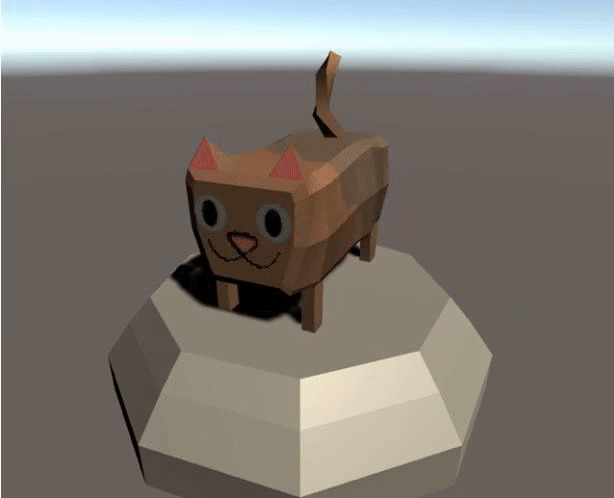
\includegraphics[width=\textwidth]{img/cat1.jpg}
        \end{subfigure}
        \hfill
        \begin{subfigure}[b]{0.24\textwidth}
            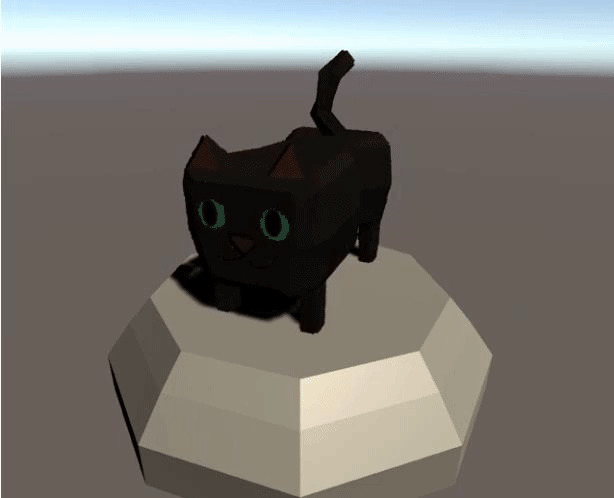
\includegraphics[width=\textwidth]{img/cat2.jpg}
        \end{subfigure}
        \hfill
        \begin{subfigure}[b]{0.24\textwidth}
            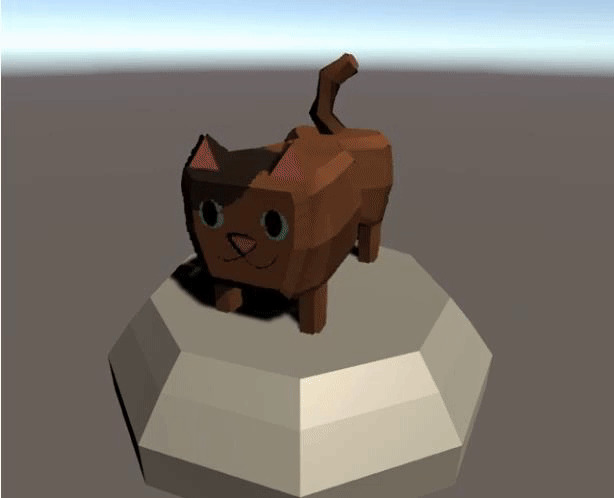
\includegraphics[width=\textwidth]{img/cat3.jpg}
        \end{subfigure}
        \hfill
        \begin{subfigure}[b]{0.24\textwidth}
            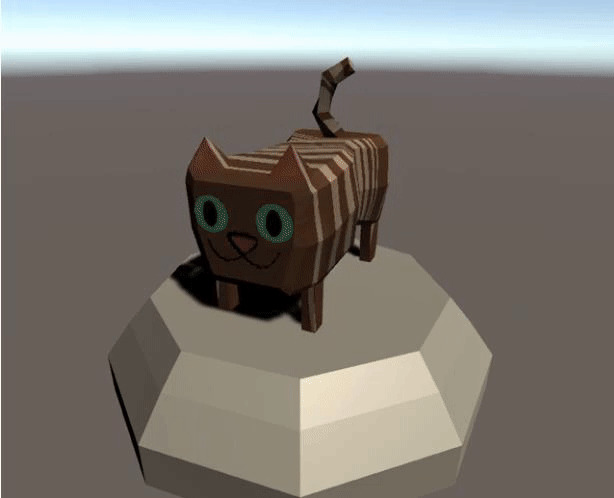
\includegraphics[width=\textwidth]{img/cat4.jpg}
        \end{subfigure}
        \caption{Modelo 3D de un gato en el que se elige semi-aleatoriamente los parámetros del pelaje. Imagen obtenida de \cite{collins2017}}
    \end{center}
\end{figure}

\subsubsection{¿Dónde y para qué se utiliza la PCG?}

La \acrshort{pcg} no solo tiene cabida en el ámbito de los videojuegos. Desde hace décadas se ha utilizado en juegos de mesa de rol (\acrshort{rol} por su sigla en inglés, \acrlong{rol}), en el cine o incluso para componer música.\\

Probablemente el ejemplo más conocido de \acrshort{rol} sea Dragones y Mazmorras (\acrshort{dyd} por su sigla en inglés, \acrlong{dyd}). En 1976, TSR Hobbies lanzó \say{\textit{Dungeon geomorphs}}, un conjunto de baldosas que permitía crear de manera procedimental gran variedad de mazmorras, similar al de la figura \ref{fig:dyd}. Las baldosas estaban diseñadas de tal modo que permitía conectar unas con otras con facilidad, cumpliendo con el objetivo principal de la \acrshort{pcg}, y es el de generar contenido jugable. Es interesante como ya en aquel entonces las instrucciones de uso de \say{\textit{Dungeon geomorphs}} invitaba al usuario a anotar el resultado obtenido con las baldosas y a realizar las modificaciones que creyese convenientes, introduciendo un elemento de vital importancia, y es la posibilidad del usuario de intervenir en el proceso y modificar el contenido generado procedimentalmente. Otro gran ejemplo de aleatoriedad guiada es la generación de encuentros y de mazmorras que también presenta \acrshort{dyd}, en su guía \say{\textit{Advanced Dungeons \& Dragons}}, utilizando lanzamientos de dados y tablas de contenido \cite{smith2015}.\\

\begin{figure}[H]
    \begin{center}
        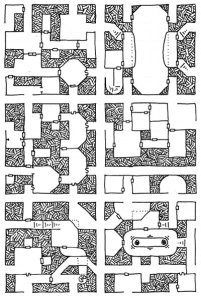
\includegraphics[scale=3, angle =90 ]{img/dungeon_geo.jpg}
        \caption{Conjunto de baldosas similar a los lanzados por TSR Hobbies en 1976. Imagen obtenida de \cite{dungeonTiles}.}
        \label{fig:dyd}
    \end{center}
\end{figure}

Un uso menos conocido de la \acrshort{pcg} es el de la generación de música y sonido. Un ejemplo de este uso es el artista Brian Eno, quién popularizó el término \say{\textit{generative music}} \cite{eno1996}. Un ejemplo más cercano es el que nos da Chister Kaitila en su breve tutorial \say{\textit{Procedural Music Generation}}, creado para la PROCJAM 2017, en el que define varias reglas para generar música procedimentalmente dónde compara la música con mazmorras y las frases musicales con las habitaciones de la mazmorra \cite{kaitila2017}.

\newpage
Fuera del mundo de los juegos, un campo en el que el uso de técnicas de \acrshort{pcg} es más frecuente de lo que podría parecer inicialmente es el cine. MASSIVE \cite{massive} es un software de generación procedimental que se creó originalmente para la trilogía del Señor de los Anillos que permite añadir miles de individuos a una escena, reduciendo el trabajo de meses a días \cite{collins2017}.\\

Este software se ha usado en multitud de películas y series como \textit{Avatar (2009)}, en la que se añadió árboles y plantas a las vastas selvas de Pandora; \textit{Guerra Mundial Z (2013)}, en la que se simularon las hordas de no-muertos o se añadió extras a las escenas tomadas en el portaaviones; \textit{La Gran Muralla (2016)}, en la que se simularon escenas con más de 300 mil criaturas; el capítulo titulado \say{\textit{La Batalla de los Bastardos}}\textit{ (2016)} de la serie \textit{Juego de Tronos}, en el que se simuló los choques de ambos ejércitos, incluyendo infantería y caballería, serie de la que podemos ver una escena antes y después de aplicar este software en la figura \ref{fig:massive}.\\

El uso de este software ha permitido un ahorro de tiempo colosal en el desarrollo de estas y muchas más obras cinematográficas, ya sea generando y simulando el comportamiento de grupos multitudinarios de entidades o dando vida a escenas en las que si no hubiera sido por este tipo de técnicas, hubiese requerido de una mayor inversión de dinero y esfuerzo.\\

\begin{figure}[H]
    \begin{center}
        \begin{subfigure}[b]{0.49\textwidth}
            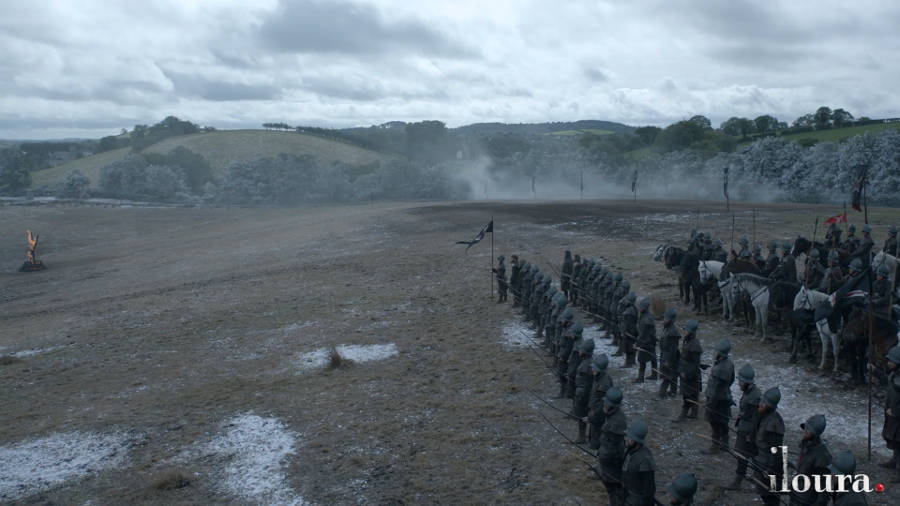
\includegraphics[width=\textwidth]{img/got_before.jpg}
            \caption{Escena antes de usar MASSIVE.}
        \end{subfigure}
        \hfill
        \begin{subfigure}[b]{0.49\textwidth}
            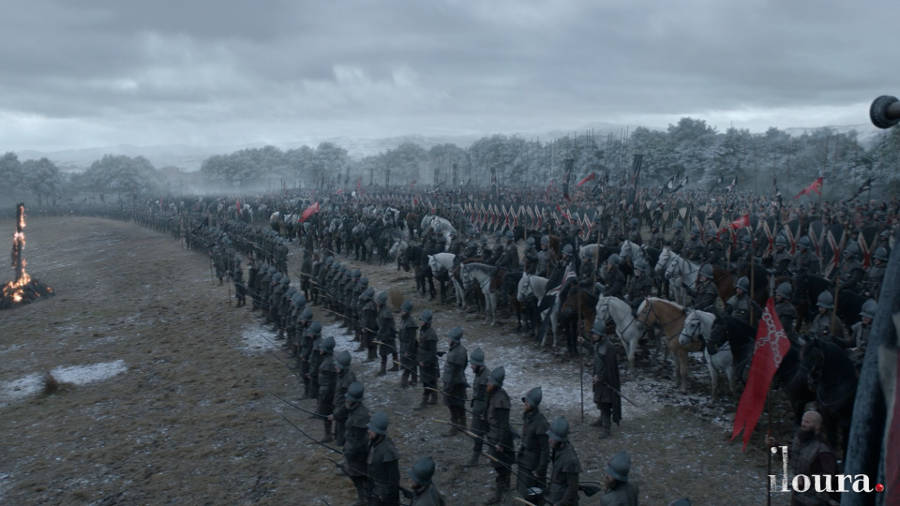
\includegraphics[width=\textwidth]{img/got_after.jpg}
            \caption{Escena tras usar MASSIVE.}
        \end{subfigure}
        \caption{Uso del software MASSIVE en la serie \textit{Juego de Tronos}. Imagen obtenida de \cite{massive}.}
        \label{fig:massive}
    \end{center}
\end{figure}

Volviendo al ámbito de los videojuegos, en sus trabajos \cite{smith2014}, \cite{smith2015} Smith habla de la utilización de métodos de \acrshort{pcg} con el fin de producir gran variedad de elementos, pasando por niveles, mapeado o texturas hasta llegar al contenido de la propia historia del videojuego. Además de la creación de contenido prácticamente ilimitado con el fin de crear una sensación de rejugabilidad en los jugadores, Smith nombra otros motivos de peso para usar \acrshort{pcg} en el desarrollo de un videojuego, ya que por ejemplo puede proporcionar un contenido que se adapte mejor al jugador. No es de extrañar que Smith centre su trabajo hacia la creación de mejores experiencias para el usuario ya que como ya hemos dicho, entiende el problema como algo más allá del campo de la \acrshort{ai}.

% ---------------------------------------------------------------------------- %

\subsection{PCG en los videojuegos}

\subsubsection{Clasificación de contenido generado procedimentalmente}

En sus trabajos sobre generación procedimental aplicada a los videojuegos Hendrikx \textit{et al.} \cite{hendrikx2013} y más tarde Barriga \cite{barriga2019} establecen una clasificación para el contenido generado procedimentalmente que se divide en las siguientes seis categorías:

\begin{enumerate}[label=(\alph*)]
    \item \textbf{Game Bits:} son las unidades más básicas de contenido de un juego. Habitualmente se trata de elementos que no interaccionan directamente con el usuario. A su vez, Hendrikx \textit{et al.} subdividen esta categoría en otros seis tipos de \textit{Game Bits}:
    
    \begin{itemize}
        \item \textit{Texturas:} se tratan de las imágenes que se utilizan para añadir detalle a las geometrías y modelos, representando habitualmente los materiales de los que están compuestos los distintos objetos del juego. En la actualidad, debido a la cantidad de esfuerzo necesario para crear texturas realistas, muchos juegos han optado por técnicas de \acrshort{pcg} para crear las texturas más generales mientras que utilizan a los artistas para generar las texturas más complejas. Podemos ver un ejemplo de una textura generada procedimentalmente en la figura \ref{fig:voronoi}.
        
        \begin{figure}[H]
            \begin{center}
                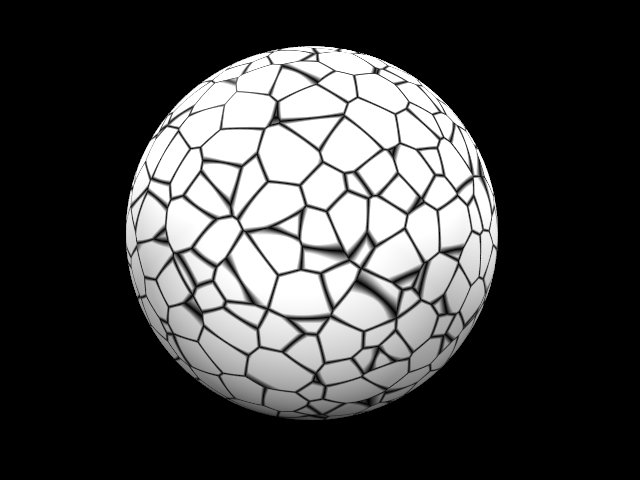
\includegraphics[scale=0.3]{img/Blender3D_VoronoiCrackle.jpg}
                \caption{Textura \textit{``fracturada''} generada procedimentalmente utilizando Teselación de Voronoi. Imagen obtenida de \cite{voronoi2007}.}
                \label{fig:voronoi}
            \end{center}
        \end{figure}
        
        \item \textit{Sonido:} tiene una función primordial en la experiencia de juego, ya que la música ayuda a establecer la atmósfera y ritmo del juego, mientras que los efectos de sonido se utilizan para dar información al usuario en función de sus acciones o de los cambios de usuario. Actualmente, los juegos dependen principalmente de clips de sonido pregrabados que se reproducen en función de los eventos del juego \cite{manocha2009}. Por otra parte, la generación procedimental aplicada a este campo no tiene una gran acogida, ya que la producción de música mediante algoritmos todavía genera animadversión entre el público y los propios compositores debido a la falsa creencia de que el ordenador es el responsable de dicha obra y no el compositor \cite{edwards2011}.
        \item \textit{Vegetación:} el uso de vegetación, además de su componente claramente visual, puede interactuar con el jugador ya sea sirviendo como lugar de cobertura o dando información al mismo, creando entornos realistas e inmersivos. Podemos ver un ejemplo de varios árboles generados procedimentalmente en la figura \ref{fig:arboles}.
        
        \begin{figure}[H]
            \begin{center}
                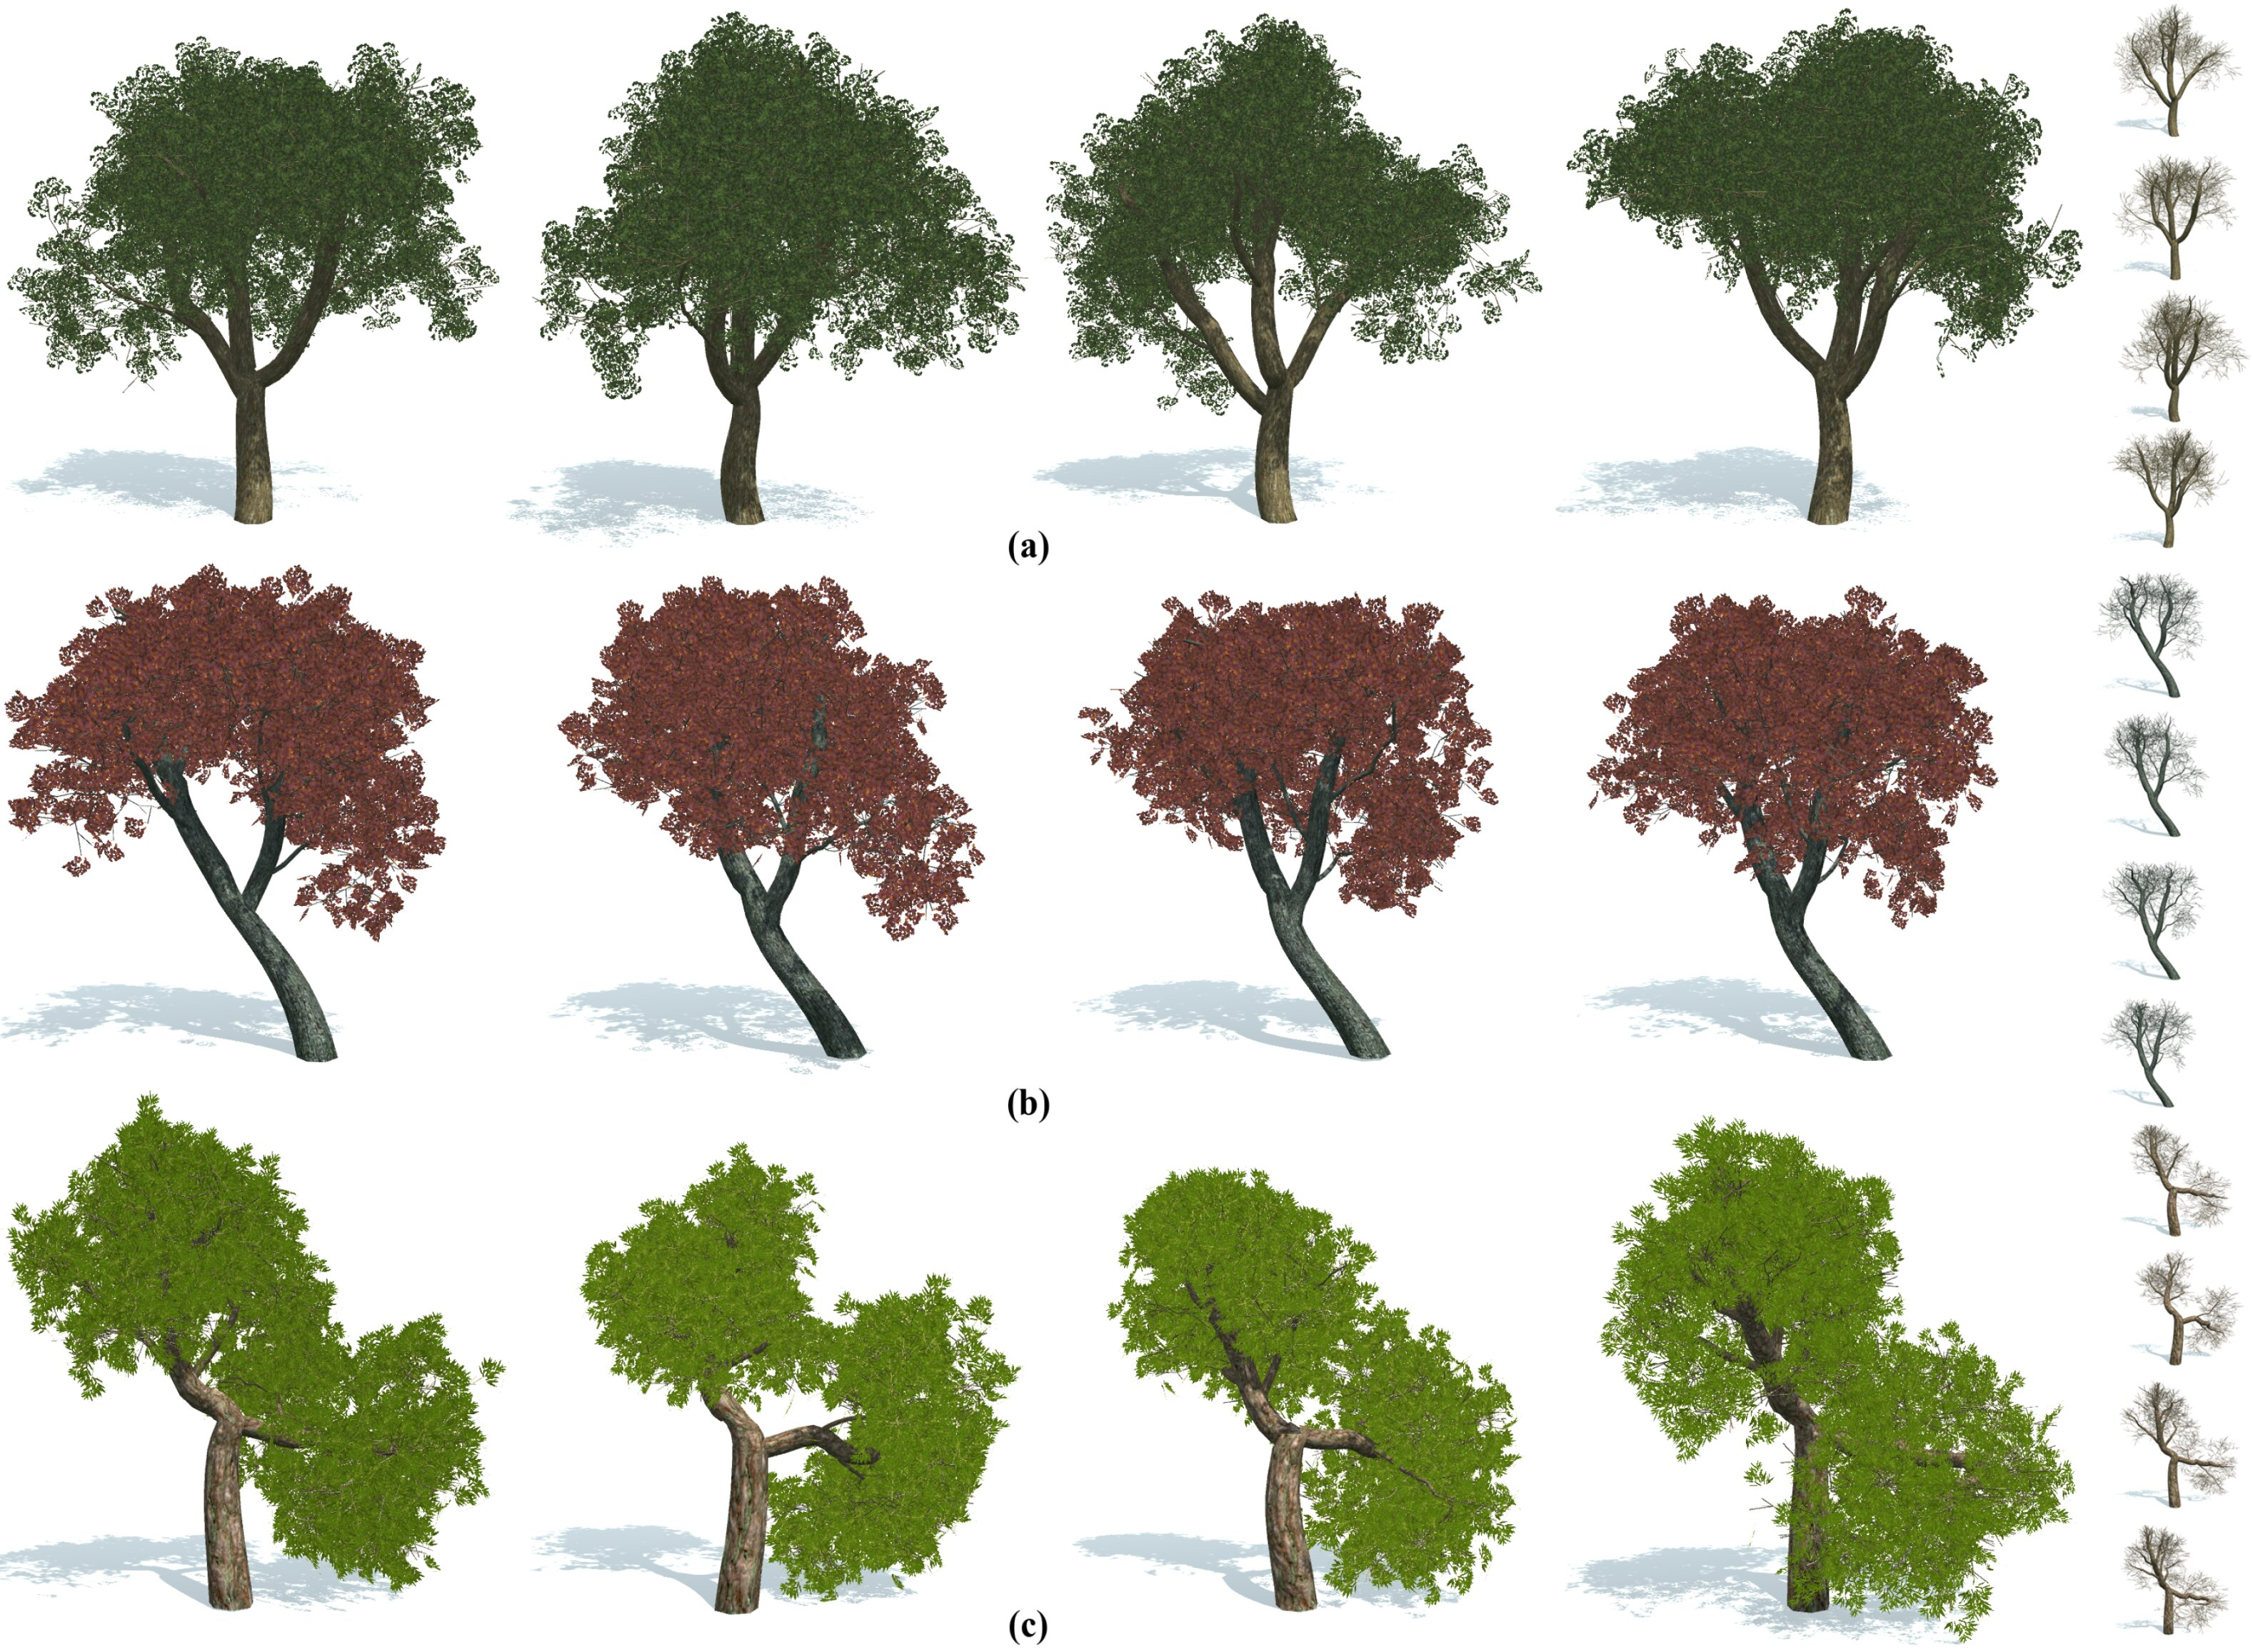
\includegraphics[scale=0.08]{img/tree-models.jpg}
                \caption{Diversos modelos de árboles generados utilizando el algoritmo procedimental propuesto por Jinmo Kim. Imagen obtenida de \cite{kim2016}.}
                \label{fig:arboles}
            \end{center}
        \end{figure}        
        
        \item \textit{Edificaciones:} al igual o más que la vegetación, los edificios ayudan a dar información al jugador del mundo que les rodea, siendo necesaria variedad en la generación de los mismos para mantener la inmersión del jugador.
        \item \textit{Comportamiento:} refiriéndose al modo en el que los objetos interaccionan entre sí y con el entorno que les rodea. Los comportamientos generados procedimentalmente permiten crear la ilusión de un entorno complejo.
        \item \textit{Elementos:} al igual que el resto de \textit{Game Bits}, los elementos como son el agua, el fuego, el viento o la tierra se utilizan para crear un entorno más realista. Con los avances computacionales y de modelado, estos han pasado de tener un papel meramente decorativo a una representación realista de los mismos y como interactúan con el mundo.
    \end{itemize}
    
    \item \textbf{Game Space:} es el entorno en el que el juego se desarrolla, en el que Hendrikx \textit{et al.} \cite{hendrikx2013} solo consideran como \textit{Game Space} a las zonas uni-, bi-, o tri-dimensionales de nuestro juego en las que están situados elementos con una posición y dirección relativa.
    
    \begin{itemize}
        \item \textit{Mapeado:} mientras Hendrikx \textit{et al.} \cite{hendrikx2013} hablan tanto de mapeado interior como exterior, Barriga \cite{barriga2019} lo simplifica unificando ambas categorías en una sola. Un ejemplo sería una mazmorra de un dungeon-crawler\footnote{Son juegos que consisten en recorrer una mazmorra, habitualmente recogiendo botín y eliminado enemigos.} como el juego \textit{Darkest Dungeon} que genera procedimentalmente la distribución y contenido de las habitaciones de la mazmorra que debe recorrer el jugador, como se puede observar en la figura \ref{fig:darkdungeon}.
        
        \begin{figure}[H]
            \begin{center}
                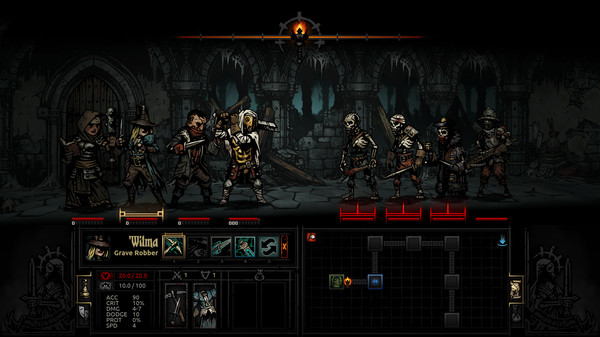
\includegraphics[scale=0.65]{img/darkest.jpg}
                \caption{En el juego \textit{Darkest Dungeon}, la distribución y contenido de la mazmorra se genera cada vez que entramos en ella. Imagen obtenida de \cite{redhook}.}
                \label{fig:darkdungeon}
            \end{center}
        \end{figure}   
        
        \item \textit{Terreno:} incluyendo elementos como ríos, lagos, mares, montañas, barrancos, grutas, etc. al igual que otros como podrían ser las zonas de teletransporte. Un ejemplo es la generación del terreno en el juego \textit{No Man's Sky}, juego en el que cada planeta que visitemos contará con distintos elementos geográficos.
    \end{itemize}
    
    \item \textbf{Game Systems:} se trata de la simulación de entornos más complejos que los representados en la categoría anterior. Un buen sistema consigue crear juegos más realistas y creíbles, por lo que son más atractivos para el consumidor. En este caso, dividimos esta categoría en cuatro tipos:
    
    \begin{itemize}
        \item \textit{Entornos urbanos:} el principal enfoque para la generación procedimental de grandes grupos de edificios primero pasa por generar las ya mencionadas redes de carreteras para a continuación generar los edificios.
        \item \textit{Comportamiento de entidades:} por último, es necesario crear entornos en los que la interacción de las distintas entidades entre sí y el jugador sean realistas y parezcan vivos. El uso de personajes no jugables (\acrshort{npc} por su sigla en inglés, \acrlong{npc}) es una de las herramientas más potentes de cara a crear estos entornos inmersivos, ya que no solo es importante una interacción realista del jugador con el resto de elementos del juego. Un claro ejemplo de situación en la que los algoritmos procedimentales pueden lograr un resultado realista es en los patrones de movimiento de grupos de individuos, como ocurre en el videojuego \textit{ S.T.A.L.K.E.R.: The Shadow of Chernobyl} \cite{amato2017}.
        \item \textit{Ecosistemas:} definen la manera en la que interaccionan flora y fauna en base a una serie de algoritmos y reglas. Esto nos permite crear sistemas en los que exista una evolución de los individuos, una definición de sus hábitats o cadenas tróficas realistas. Podemos ver un ejemplo de un ecosistema compuesto por flora y fauna generados procedimentalmente en la figura \ref{fig:noman}.
        
        \begin{figure}[H]
            \begin{center}
                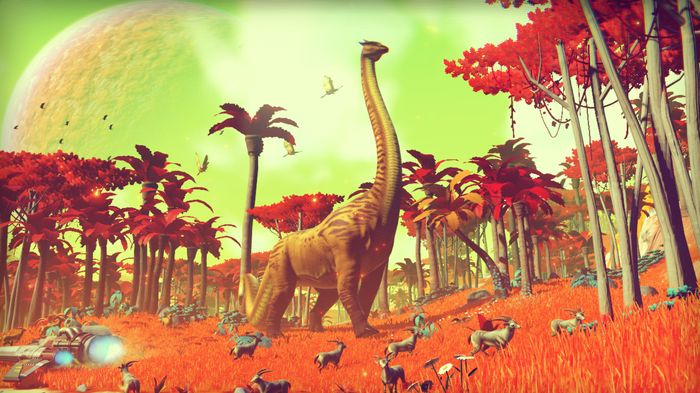
\includegraphics[scale=0.4]{img/no-mans-sky.jpg}
                \caption{En el juego \textit{No Man's Sky}, los ecosistemas de cada planeta son generados procedimentalmente. Imagen obtenida de \cite{grendel-games}.}
                \label{fig:noman}
            \end{center}
        \end{figure}    
        
        \item \textit{Redes de carreteras:} son la estructura básica de comunicación entre los distintos puntos de interés de nuestro mapeado. La dificultad de generar redes de carreteras de manera procedimental es la búsqueda de equilibrio entre la aleatoriedad y el cumplir con una estructura lógica en la disposición de nuestros elementos. Este será uno de los tipos de contenido que generaremos en este proyecto.
    \end{itemize}
    
    \item \textbf{Game Scenarios:} en este apartado encontraríamos los tres niveles anteriores organizados de tal modo que forman planes coherentes o secuencias de eventos. Podemos distinguir claramente cuatro categorías en las que dividir los \textit{Game Scenarios}:
    
    \begin{itemize}
        \item \textit{Guiones gráficos:} principalmente utilizan el formato de viñeta y sirven de ayuda para guiar a los desarrolladores o al propio jugador. En función del modo en el que se usen podremos incluirlo en esta categoría o en la categoría \textit{Derived Content}.
        \item \textit{Historia:} normalmente es la pieza fundamental para crear historias que mantengan al jugador motivado, establecer un sentido lógico a los eventos del juego y proporcionar la meta principal que debe alcanzar nuestro jugador.
        \item \textit{Puzzles:} son problemas a los que el jugador debe encontrar una solución basada en sus conocimientos previos o en la información obtenida al explorar el entorno. Dependiendo del tamaño del problema que se plantee y de la experiencia previa del jugador variará la dificultad asociada al mismo. Un gran ejemplo, visible en la figura \ref{fig:minimotor} es el juego \textit{Mini Metro}, que genera procedimentalmente los niveles, generando puzzles distintos cada vez que se juega y teniendo como objetivo alcanzar la máxima puntuación posible.
        
        \begin{figure}[H]
            \begin{center}
                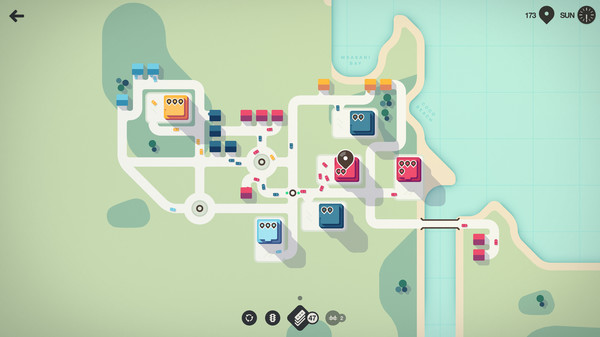
\includegraphics[scale=2]{img/minimotor.jpg}
                \caption{En el juego \textit{Mini Motorways}, la distribución de casas y centros comerciales se genera procedimentalmente. Imagen obtenida de \cite{dinosaurPolo}.}
                \label{fig:minimotor}
            \end{center}
        \end{figure}    
        
        \item \textit{Niveles:} su definición más usada es la de separador entre las distintas secuencias del juego. Son aquellas zonas jugables dónde el jugador debe ir del punto A al punto B, cumpliendo una serie de objetivos por el camino. Podemos ver un ejemplo de nivel generado procedimentalmente del juego \textit{Bad North} en la figura \ref{fig:badnor}, aplicando técnicas \acrshort{pcg} a la generación de niveles en \acrshort{3d}. Este será uno de los tipos de contenido que generaremos en este proyecto.
    \end{itemize}
    
        \begin{figure}[H]
            \begin{center}
                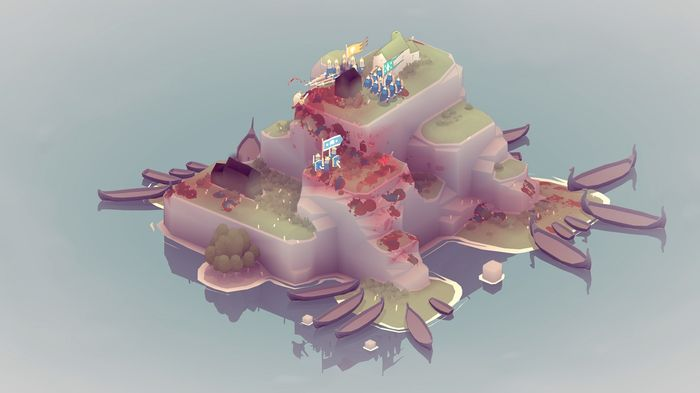
\includegraphics[scale=0.4]{img/bad_north.jpg}
                \caption{En el juego \textit{Bad North}, cada nivel se genera mediante un método conocido como colapso de la función de onda. Imagen obtenida de \cite{grendel-games}.}
                \label{fig:badnor}
            \end{center}
        \end{figure}     
    
    \item \textbf{Game Design:} son las mecánicas y reglas del juego, estableciendo lo que se puede hacer en el juego y lo que no. Tal y como definen en su trabajo Hendrikx \textit{et al.} esta categoría incluye y referencia a todo el contenido ya descrito, incluso de manera recursiva a otro contenido perteneciente al \textit{Game Design}. Todo este contenido puede ser generado automáticamente o de tal modo que proporcione herramientas a los diseñadores.
    \item \textbf{Derived Content:} definiendolo brevemente se trata del contenido que se crea paralelamente al mundo del juego, creando un gran sentido de inmersión en el jugador ya que refleja las acciones y experiencia del usuario dentro y fuera del propio juego.
\end{enumerate}

De esta clasificación en forma de pirámide debemos destacar que los elementos complejos de los niveles superiores suelen estar compuestos de los elementos más simples de los elementos inferiores. Además, debemos dejar claro que aunque algunos de estos elementos son necesarios, otros simplemente son opcionales y no tienen por qué formar parte del desarrollo de un videojuego. Debemos recalcar de nuevo la importancia de un contenido de calidad a la hora de crear entornos inmersivos para el jugador.\\

\begin{figure}[H]
    \begin{center}
        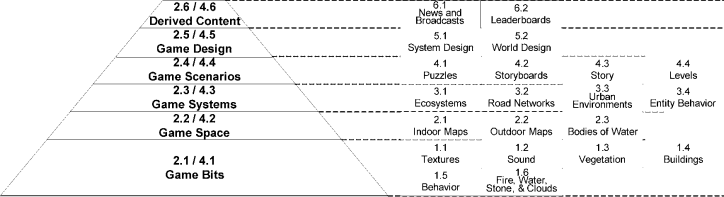
\includegraphics[scale=0.8]{img/hendrikx2013.png}
        \caption{Clasificación piramidal del contenido generado procedimentalmente. Imagen obtenida de \cite{hendrikx2013}.}
    \end{center}
\end{figure}

\subsubsection{Propiedades deseables del PCG}

Dependiendo del problema al que nos enfrentemos y el objetivo que busquemos alcanzar, los métodos de \acrshort{pcg} contaran con distintas características y propiedades. Habitualmente estas características no serán alcanzables a la vez, como ejemplo, podemos implementar un algoritmo muy rápido pero que no asegure la máxima calidad del contenido generado. En el libro de Shaker \textit{et al.} \cite{shaker2016} hablan de las siguientes características deseables de los algoritmos de \acrshort{pcg}:

\begin{itemize}
    \item \textbf{Velocidad:} refiriéndose al tiempo que tarda el algoritmo en generar contenido. Dependiendo del problema, podríamos necesitar una solución en milésimas de segundo a poder permitirnos esperar durante horas.
    \item \textbf{Fiabilidad:} refiriéndose a la precisión con la que garantiza el algoritmo que el contenido generado es de calidad. Mientras que en ocasiones necesitaremos que el contenido no contenga errores, por ejemplo, en la generación de un laberinto, en otras ocasiones, no nos importará sacrificar parte de la calidad del contenido a cambio de velocidad, por ejemplo, en la generación de vegetación.
    \item \textbf{Controlabilidad:} refiriéndose a la posibilidad de una persona u otro algoritmo de modificar o condicionar los resultados obtenidos por el método de \acrshort{pcg}.
    \item \textbf{Diversidad:} refiriéndose a la capacidad de generar contenido variado y que no se base en simples variaciones. Normalmente no es trivial conseguir diversidad sin afectar a la calidad del contenido.
    \item \textbf{Credibilidad:} refiriéndose a la capacidad de imitar al contenido generado por humanos y que no parezca que el contenido generado ha sido creado utilizando algoritmos de \acrshort{pcg}.
\end{itemize}

\subsubsection{Métodos de generación de contenido}

En cuanto a la clasificación de los distintos algoritmos no existe un convenio de categorías en las que dividirlos. Algunos autores como Shaker \textit{et al.} \cite{shaker2016} definen una taxonomía dividida en siete categorías, otros como Hendrikx \textit{et al.} \cite{hendrikx2013} dividen los métodos en seis categorías y otros como Barriga \cite{barriga2019} simplifica las taxonomías anteriormente propuestas a tres categorías.\\

En nuestro caso nos quedaremos con la clasificación propuesta por Barriga ya que, al estar simplificada a tres categorías, facilita una primera aproximación a la generación procedimental de contenidos.\\

\begin{table}[H]
    \centering
    \caption{Clasificación de métodos de generación de contenido con ejemplos.}
    \begin{tabular}{|l|l|}
    \hline
    Categoría                         & Métodos de PCG                                                                                                                                          \\ \hline
    Métodos tradicionales             & \begin{tabular}[c]{@{}l@{}}Generación de números semi-aleatoria\\ Generación basada en fractales y ruido\\ Generación basada en gramáticas\end{tabular} \\ \hline
    Métodos basados en búsqueda       & Algoritmos evolutivos                                                                                                                                   \\ \hline
    Métodos de aprendizaje automático & \begin{tabular}[c]{@{}l@{}}Redes neuronales recursivas\\ Autoencoders\\ Modelos de Markov\end{tabular}                  \\ \hline
    \end{tabular}
\end{table}

\newpage

\paragraph{Métodos tradicionales}

Por norma general, son los métodos más simples y rápidos. Dependiendo del contenido que queramos generar ciertos métodos brillan frente al resto.\\ 

Los primeros métodos llevados a la industria de los videojuegos es la generación semi-aleatoria de números, utilizada principalmente para la generación de laberintos y mazmorras. Al ser habitualmente deterministas nos permiten representar el contenido generado mediante una semilla\footnote{Número que representa los pasos realizados por nuestro algoritmo y nos permite replicarlos.} que generaría siempre el mismo contenido.\\

Otro ejemplo es el uso de generación basada en fractales y ruido para generar texturas o paisajes. Esto se debe a que los resultados de estos métodos generan resultados similares a los de los procesos naturales, generando una sensación orgánica. Un ejemplo es el ruido Perlin \cite{perlin} que se usa por ejemplo para generar nubes o texturas de mármol.\\

Por último, los métodos de generación basados en gramáticas son los más utilizados para generar vegetación, aunque también pueden usarse para generar otro contenido como ciudades o niveles de un juego de plataformas. Un ejemplo podría ser el desarrollado por Sportelli \textit{et al.} \cite{sportelli2014} en el que generan los niveles del juego \textit{The Ball: Lost in Space} utilizando una gramática.\\

\begin{figure}[H]
    \begin{center}
        \begin{subfigure}[b]{0.3\textwidth}
            \centering
            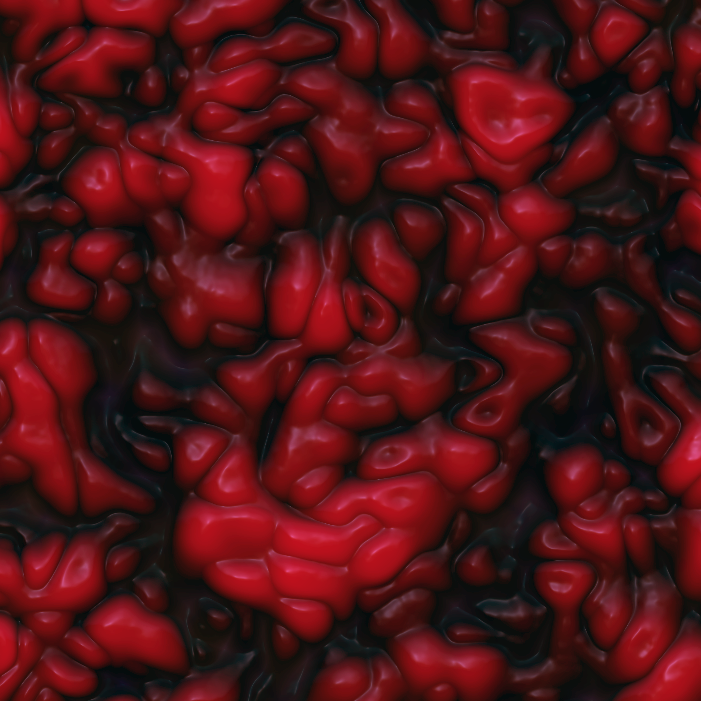
\includegraphics[scale=0.164]{img/redPerlin.png}
            \caption{Tejido orgánico.}
        \end{subfigure}
        \hfill
        \begin{subfigure}[b]{0.3\textwidth}
            \centering
            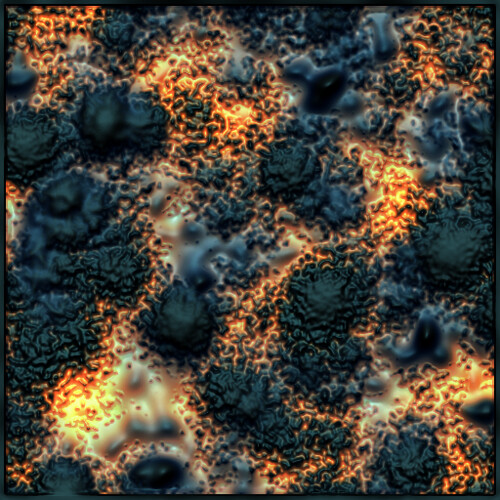
\includegraphics[scale=0.2305]{img/lavaPerlin.jpg}
            \caption{Terreno volcánico.}
        \end{subfigure}
        \hfill
        \begin{subfigure}[b]{0.3\textwidth}
            \centering
            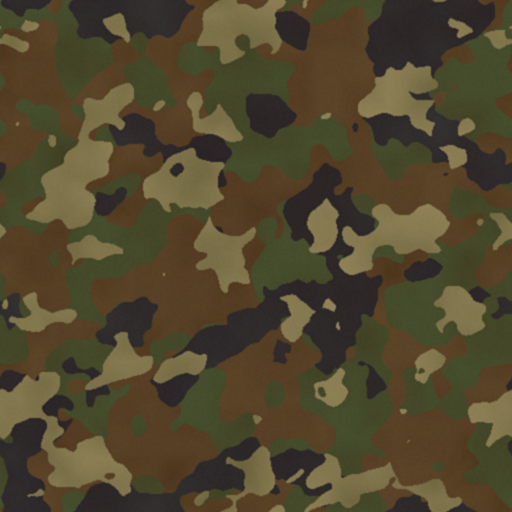
\includegraphics[scale=0.224]{img/camufaje.png}
            \caption{Patrón de camuflaje.}
        \end{subfigure}
        \caption{Texturas generadas utilizando ruido Perlin. Imágenes obtenidas de \cite{redPerlin}, \cite{lavaPerlin} y \cite{camuflajePerlin}.}
    \end{center}
\end{figure}

\paragraph{Métodos basados en búsqueda}
Estos métodos se basan en la generación de contenido seguida de una evaluación del mismo, puntuando su calidad. En estos métodos podemos identificar tres componentes: la representación del espacio, la función de evaluación y el algoritmo de búsqueda.

\begin{itemize}
    \item \textbf{Representación del espacio:} dependiendo del contenido generado y de la forma de generar dicho contenido, este contará con una representación. Las formas de representar estos datos pasan por vectores, matrices, árboles e incluso por un diseño específico para nuestro problema.
    \item \textbf{Función de evaluación:} será la encargada de evaluar la calidad de las soluciones obtenidas. Esta evaluación puede ser desde una función simple de combinaciones lineales de características (por ejemplo, en un laberinto, cuantos cruces tiene, si tiene caminos cerrados, etc.) o funciones complejas que utilicen modelos matemáticos para su optimización, como en el caso de las redes neuronales.
    \item \textbf{Algoritmo de búsqueda:} es el encargado de realizar una búsqueda en nuestra representación del espacio apoyándose en la función de evaluación para escoger los mejores individuos del espacio. Tal y como refleja Togelius \textit{et al.} \cite{togelius2011} el método más utilizado como algoritmo de búsqueda son los algoritmos evolutivos, aunque también se utilizan otros métodos como enfriamiento simulado, búsqueda local o cualquier otro tipo de metaheurística \cite{molina2020}.
\end{itemize}

Un gran ejemplo de aplicación de métodos basados en búsqueda para generar contenido es el experimento llevado a cabo por Togelius \textit{et al.} \cite{togelius2007} en el que generan de manera evolutiva circuitos para un juego de carreras.

\paragraph{Métodos de aprendizaje automático}

Recientemente diversos métodos de aprendizaje automático han demostrado ser capaces de generar contenido de juegos. Algunos ejemplos exitosos son la generación de nuevos niveles del videojuego Super Mario usando redes neuronales recursivas por Summerville \& Mateas \cite{summerville2016}, usando autoencoders por Jain \textit{et al.} \cite{jain2016} o usando modelos de Markov por Snodgrass \& Ontañón \cite{snodgrass2017}. Como se puede observar en el trabajo de Barriga \cite{barriga2019} y en los ejemplos recién expuestos, los métodos de aprendizaje automático se usan principalmente para la generación de niveles.

\begin{figure}[H]
    \begin{center}
        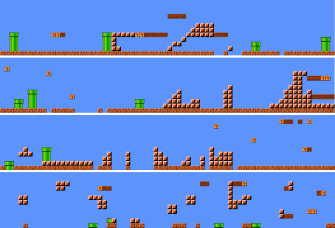
\includegraphics[scale=0.775]{img/mario.png}
        \caption{Niveles del videojuego Super Mario generados utilizando Modelos de Markov. Imagen obtenida de \cite{snodgrass2017}.}
    \end{center}
\end{figure}

% ---------------------------------------------------------------------------- %

\subsubsection{Recorrido histórico del uso de la PCG}

Los métodos de generación procedimental de contenido no solo se han usado en el ámbito de los videojuegos en la última década sino que su aplicación aparece ya a principio de la década de los 80. En este breve recorrido histórico seguiremos el primer capítulo del libro de Shaker \textit{et al.} \cite{shaker2016} y el trabajo de Amato \cite{amato2017}, sacando información sobre juegos que usan generación procedimental tanto de la web \textit{The Gamer} \cite{glenn2021} como de Wikipedia \cite{listWiki}. Además, podemos añadir una mención especial a \textit{Everything Procedural} \cite{EP}, la conferencia anual sobre generación procedimental aplicada a videojuegos.

\begin{table}[H]
    \centering
    \caption{Relación de videojuegos que usan PCG.}
    \begin{tabular}{|l|l|l|}
    \hline
    Videojuego & Lanzamiento & Contenido generado procedimentalmente \\ \hline
    Rogue      & 1980        & Niveles ASCII  \\ \hline
    Elite      & 1984        &     Planetas y galaxias   \\ \hline
    \textit{Saga} Civilation     & 1991-2018        & Niveles \acrshort{2d} y \acrshort{3d}   \\ \hline
    \textit{Saga} X-Com     & 1993-2016        &  Niveles \acrshort{2d} y \acrshort{3d}  \\ \hline
    Diablo     & 1996        & Niveles \acrshort{2d} y recompensas     \\ \hline
    KKrieger     & 2004        & Mallas, texturas y música     \\ \hline
    Dwarf Fortress & 2006 & Mapeado y ecosistemas \\ \hline
    The Elder Scrolls IV: Oblivion     & 2006        & Vegetación     \\ \hline
    Spelunky     & 2008        & Niveles \acrshort{2d}  \\ \hline
    Spore     & 2008        & Terreno, planetas, criaturas y animaciones \\ \hline
    \textit{Saga} Batman: Arkham     & 2009-2015        & Vegetación   \\ \hline
    \textit{Saga} Borderlands     & 2009-2019        & Armas   \\ \hline
    Left 4 Dead 2     & 2009        & Dificultad adaptativa   \\ \hline
    Minecraft     & 2011        & Mundo \acrshort{3d}      \\ \hline
    Elite: Dangerous     & 2015        & Planetas y galaxia \\ \hline
    Rogue Legacy &	2011 & Niveles \acrshort{2d} \\ \hline
    Terraria &	2011 & Mundo \acrshort{2d} \\ \hline
    \textit{Saga} The Binding of Isaac &	2011-2021 & Niveles \acrshort{2d}  \\ \hline
    Don't Starve &	2013 & Mundo \acrshort{2d} \\ \hline
    Crypt of the NecroDancer &	2015 & Niveles \acrshort{2d} \\ \hline
    Mini Metro &	2015 & Localización objetivos y recursos, y audio \\ \hline
    Darkest Dungeon & 2016 & Niveles \acrshort{2d} \\ \hline
    Enter the Gungeon & 2016 & Niveles \acrshort{2d} \\ \hline
    No Man's Sky & 2016 & Planetas, recursos, ecosistemas, criaturas, etc.  \\ \hline
    Bad North & 2018 & Niveles \acrshort{3d}  \\ \hline
    Into The Breach & 2018 & Niveles \acrshort{2d}\\ \hline
    Mini Motorways & 2019 & Localización objetivos y recursos \acrshort{3d} \\ \hline
    Townscaper & 2020 & Niveles \acrshort{3d} \\ \hline
    Valheim & 2021 & Mundo \acrshort{3d} \\ \hline
    \end{tabular}
\end{table}

\newpage

En 1980 se publicó \textit{Rogue} \cite{wichman1997}, uno de los primeros \textit{dungeon-crawlers} y el considerado ancestro de los juegos \textit{Rogue-like}\footnote{La traducción literal es "que se parece a Rogue", de ahí el nombre de esta categoría.} Esta categoría de juegos siempre utiliza algún tipo de generación procedimental ya que, tal y como ya pasaba en \textit{Rogue}, los niveles se generan aleatoriamente cada vez que comienza el juego.\\

\begin{figure}[H]
    \begin{center}
        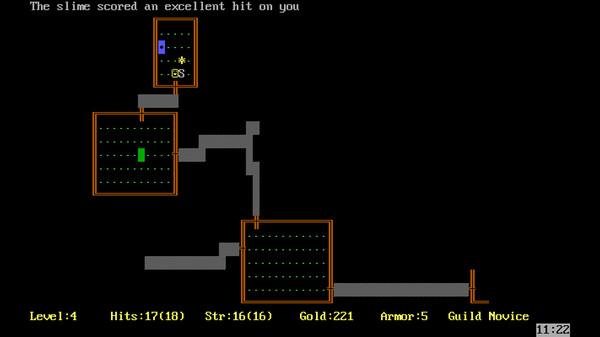
\includegraphics[scale=0.37]{img/rogue.jpg}
        \caption{Mazmorra generada procedimentalmente del videojuego \textit{Rogue}. Imagen obtenida de \cite{epyx}.}
    \end{center}
\end{figure}

Unos años más tarde, en 1984, se publicó \textit{Elite} \cite{braben2007} que estableció una solución para las capacidades limitadas de los ordenadores de 8 bits, generando procedimentalmente 256 planetas distribuidos en 8 galaxias mediante una semilla. Más tarde, en 2014 se publicó \textit{Elite: Dangerous}, una versión moderna del juego que usando \acrshort{pcg} te permite explorar una galaxia compuesta por 400 mil millones de sistemas estelares, números solo alcanzables gracias a la generación procedimental, como bien señala Amato \cite{amato2017}, ya que suponiendo que un sistema solar ocupase solamente 1\acrshort{KB}, el sistema representando en el juego ocuparía 40\acrshort{TB}.\\

\begin{figure}[H]
    \begin{center}
        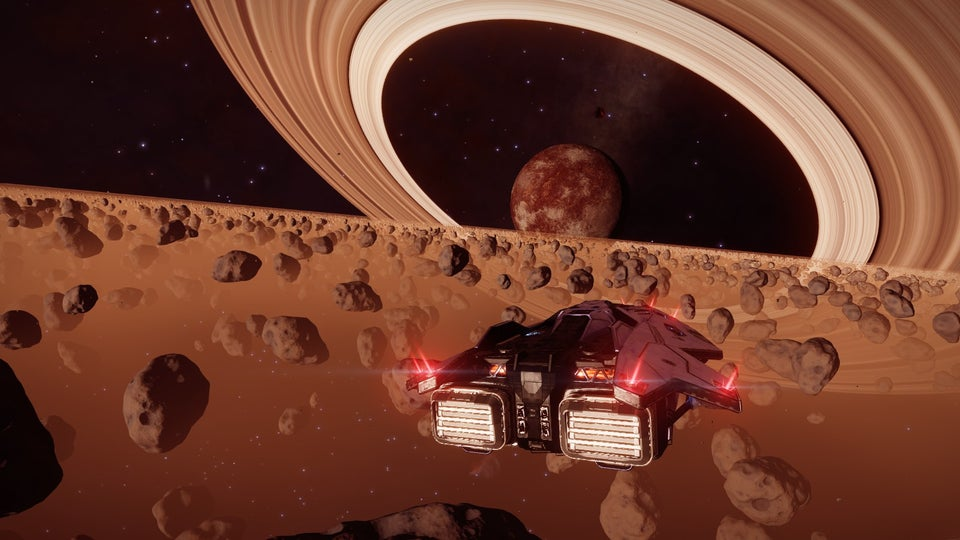
\includegraphics[scale=0.23]{img/elitedangerous.jpg}
        \caption{Planeta y cinturón de asteroides del videojuego \textit{Elite: Dangerous}. Imagen obtenida de \cite{eliteDangerous}.}
    \end{center}
\end{figure}

Más tarde, cuando comenzaron a desaparecer las limitaciones de espacio, aparecieron juegos como Diablo \cite{diablo}, un \textit{Rogue-like} híbrido que no solo generaba sus niveles procedimentalmente sino que implementó un sistema de recompensas que se generaban en el momento, sistema que se ha visto posteriormente en otros títulos como la saga de \textit{Borderlands}.\\

Poco a poco comenzó a usarse técnicas de \acrshort{pcg} con el fin de generar contenido más allá del nivelado del juego. Por ejemplo, el videojuego \textit{KKrieger} \cite{kosh} es un juego en \acrshort{3d} en primera persona publicado en 2004 que ocupa menos de 100\acrshort{KB} debido a que utiliza generación procedimental para crear las mallas de los modelos, las texturas e incluso la música.

\begin{figure}[H]
    \begin{center}
        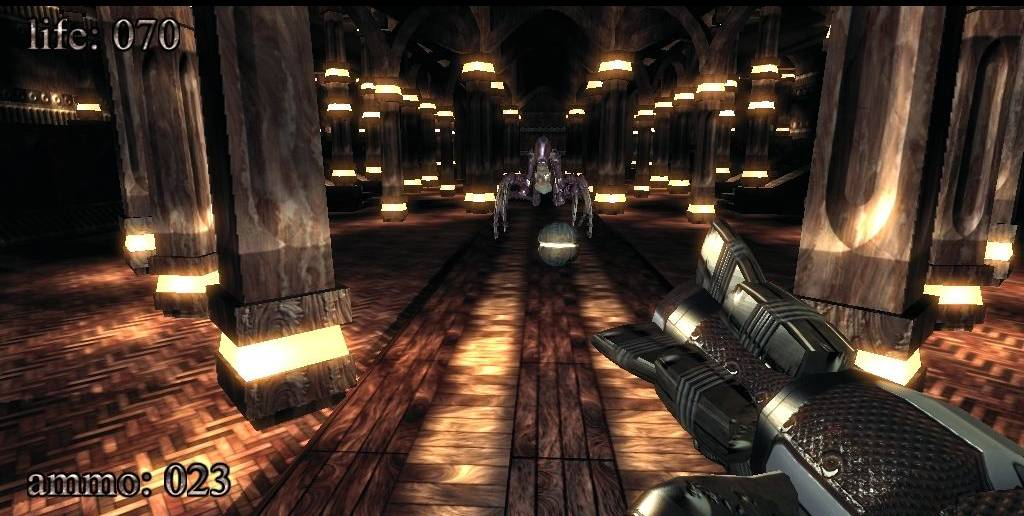
\includegraphics[scale=0.3]{img/kkrieger.jpg}
        \caption{Mazmorra generada procedimentalmente del videojuego \textit{Kkrieger}. Imagen obtenida de \cite{chirinea}.}
    \end{center}
\end{figure}

Aunque si hablamos de videojuegos que utilizan técnicas de \acrshort{pcg} como base fundamental de su jugabilidad no podemos evitar hablar de \textit{Spore} \cite{spore}, juego lanzado en 2008 en el que se generaba planetas, criaturas, terreno y otros elementos como las animaciones de las criaturas que se generan al momento, y de \textit{No Man's Sky} \cite{nomansky}, juego lanzado en 2016 que nos permite visitar 18 trillones de planetas ya que genera prácticamente la totalidad de su contenido procedimentalmente.

\begin{figure}[H]
    \centering
        \begin{subfigure}[b]{0.49\textwidth}
            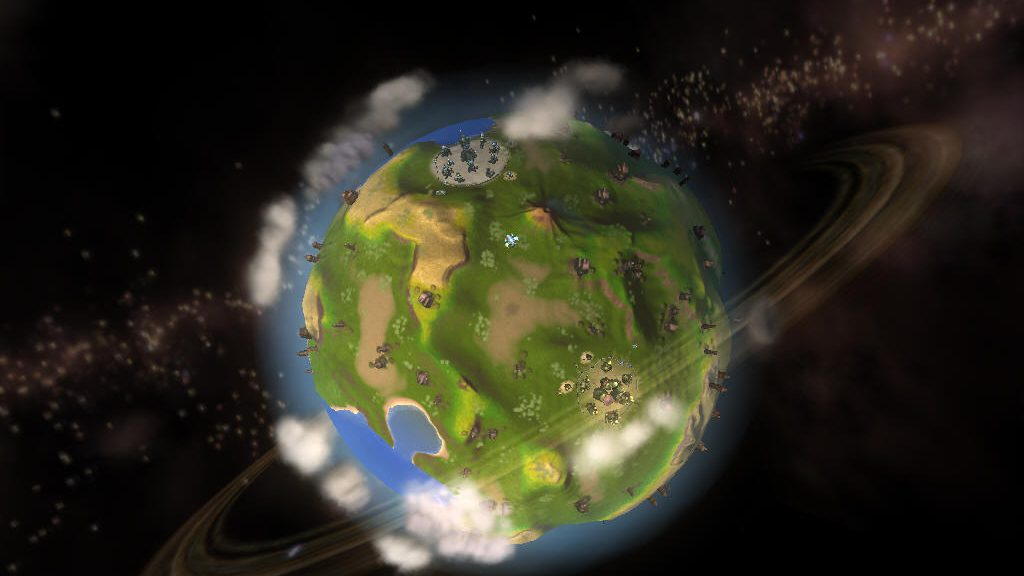
\includegraphics[width=\textwidth]{img/spore.jpg}
            \caption{Planeta del videojuego \textit{Spore}.}
        \end{subfigure}
        \hfill
        \begin{subfigure}[b]{0.49\textwidth}
            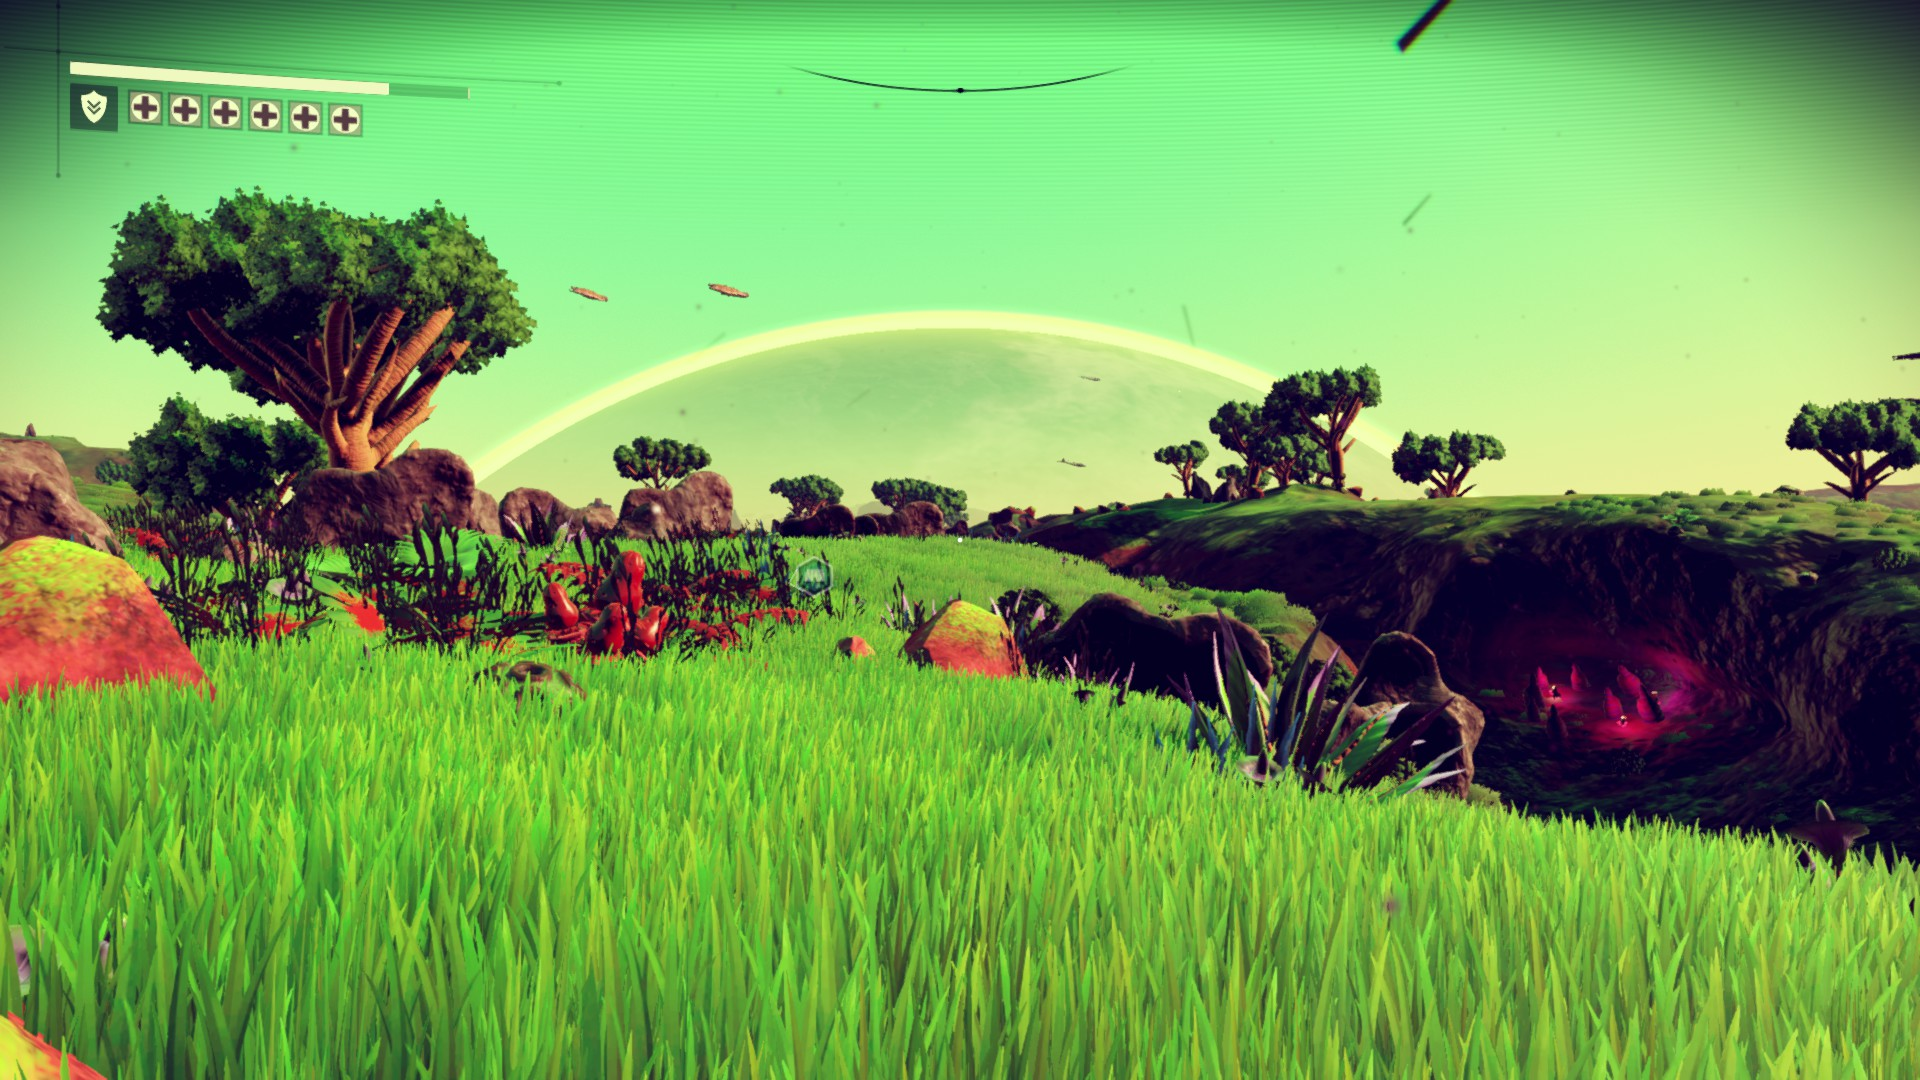
\includegraphics[width=\textwidth]{img/jake.jpeg}
            \caption{Planeta del videojuego \textit{No Man's Sky}.}
        \end{subfigure}
        \caption{Escenas de juegos que han basado elementos principales de su desarrollo en PCG. Imágenes obtenidas de \cite{spore} y \cite{jake}.}
\end{figure}

Con el tiempo se ha desarrollado incluso software específico para generar contenido especializado de manera procedimental, como ocurre con la herramienta \textit{SpeedTree} \cite{speedtree} que se ha especializado en generación y modelado de vegetación y se ha usado en juegos como la saga \textit{Batman: Arkham}, en \textit{The Elder Scrolls IV: Oblivion} o en el propio \textit{No Man's Sky}.\\

Sin embargo, aunque la generación procedimental se ha usado en diversos géneros y para generar multitud de contenido, se puede observar que dentro del mundo de los videojuegos el contenido más frecuentemente generado es el nivelado y mapeado, por ello los juegos \textit{Rogue-like} son los que mayoritariamente se benefician de y aplican técnicas de generación procedimental. Esto se puede observar en el catálogo de videojuegos que han utilizado \acrshort{pcg} como un elemento principal de su diseño.\\

Contamos con multitud de ejemplos de juegos que cumplen con esto, entre ellos, \textit{Rogue Legacy} o \textit{Darkest Dungeon}, que al más puro estilo de original \textit{Rogue} nos permite recorrer una \acrshort{2d} diferente cada vez que comencemos una nueva misión; otros como \textit{Crypt of the NecroDancer} o \textit{Into The Breach}, que combinan la rejugabilidad y variedad que aporta la generación procedimental con mecánicas ya conocidas pero novedosas en este nicho, siendo el primero un juego de ritmo y el segundo un juego de puzzles; e incluso juegos que su atractivo principal es el uso de generación procedimental, tal y como hace \textit{Townscaper} cuya jugabilidad se basa en diseñar ciudades generadas procedimentalmente.\\

\begin{figure}[H]
    \begin{center}
        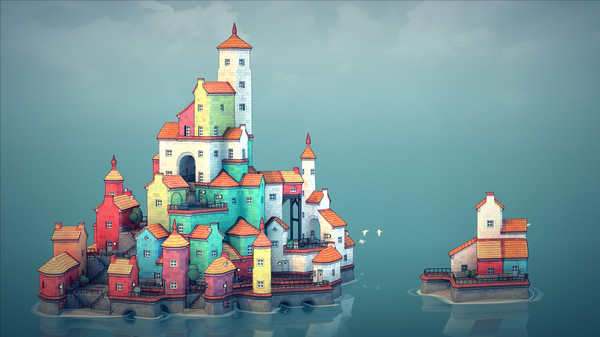
\includegraphics[scale=0.4]{img/town.jpg}
        \caption{Ciudad generada procedimentalmente por un jugador en el juego \textit{Townscaper}. Imagen obtenida de \cite{oscar}.}
    \end{center}
\end{figure}
    
    
    
    \newpage
    \section{Análisis del problema}

    En este apartado explicaremos el funcionamiento del videojuego clásico Pac-Man, las bases y componentes del juego, el diseño de los niveles y el comportamiento de los fantasmas. También haremos una propuesta que cumpla con los objetivos específicos presentados en la primera sección, centrándonos principalmente en definir los apartados del juego en los que aplicaremos \acrshort{pcg}.

\subsection{Videojuego clásico escogido: Pac-Man}

    Hemos decidido escoger para su reimplementación aplicando técnicas de generación procedimental al videojuego Pac-Man \cite{officialSitePacman}, publicado en 1980 por la empresa Bandai Namco Entertainment Inc., conocido por todo el mundo y probablemente uno de los juegos más icónicos de todos los tiempos. Desde entonces se ha publicado multitud de contenido relacionado con esta franquicia, comenzando por decenas de nuevos videojuegos basados en el juego original, pasando por merchandising e incluso otro tipo de contenido como la guía \textit{Mastering Pac-Man} \cite{uston}, escrita por Ken Uston en 1981 en la que desvelaba todos los secretos del juego.\\
    
    Debido al hito en la historia de los videojuegos que supuso Pac-Man, a que las mecánicas y funcionamiento del juego pueden suponer un reto interesante a la hora de implementarlo, a que debido a que el juego original no utilizaba técnicas de generación procedimental y que el contenido del juego es apto para generarlo procedimentalmente (especialmente los laberintos), se ha decido escoger este juego. Para esta sección seguiremos el informe realizado por Jamey Pittman \cite{pittman2015} y la guía publicada por el usuario de Steam \textit{Night Druid} \cite{druid2016}. 
    
    \begin{figure}[H]
    \centering
        \begin{subfigure}[b]{0.49\textwidth}
        \centering
            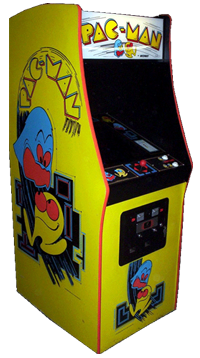
\includegraphics[width=3.3cm]{img/cabinet3.png}
            \caption{Máquina recreativa del videojuego original.}
        \end{subfigure}
        \hfill
        \begin{subfigure}[b]{0.49\textwidth}
        \centering
            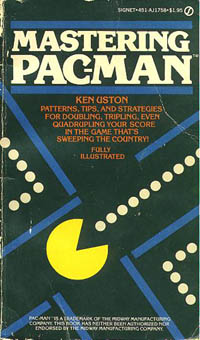
\includegraphics[width=3.3cm]{img/pbook.jpg}
            \caption{Guía escrita por Ken Uston.}
        \end{subfigure}
        \caption{Ejemplos de contenido relacionado con la franquicia de \textit{Pac-Man}. Imágenes obtenidas de \cite{pittman2015}.}
    \end{figure}

\subsubsection{Objetivo del juego}

El objetivo del juego es recorrer un laberinto comiéndonos todos los puntos situados a lo largo del mismo mientras escapamos de cuatro enemigos, los fantasmas. Si nos comemos todos los puntos, avanzamos de nivel, y si nos atrapan los fantasmas, perdemos una vida y se reiniciará la posición de Pac-Man y los fantasmas. Como ayuda contra los fantasmas, Pac-Man podrá utilizar un potenciador que le proporcionará invencibilidad y le permitirá derrotar a los fantasmas. Si derrotamos a un fantasma, volverá a su zona de inicio y reaparecerá para volver a perseguir a Pac-Man.

\subsubsection{Diseño de niveles}

El juego está compuesto por Pac-Man, el personaje amarillo; los 4 fantasmas, cada uno de un color (rojo, azul, rosa y naranja); laberinto (los pasillos y los muros), con una sección que llamaremos la ``casa'' de los fantasmas; 244 puntos y 4 potenciadores. Además, el laberinto contará con una conexión que unirá la parte derecha e izquierda del escenario, que llamaremos \textit{teletransportes}.

 \begin{figure}[H]
    \centering
        \begin{subfigure}[b]{0.4\textwidth}
        \centering
            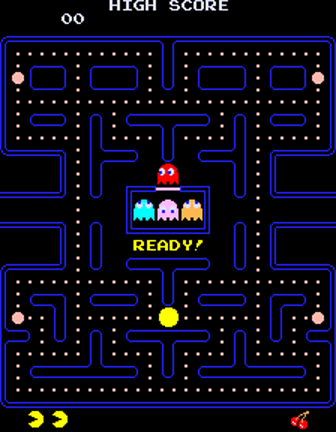
\includegraphics[width=5cm]{img/lvl1.png}
        \caption{Diseño de los niveles del 0 al 255.}
        \end{subfigure}
        \hspace{1cm}
        \begin{subfigure}[b]{0.4\textwidth}
        \centering
            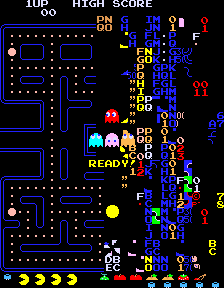
\includegraphics[width=5cm]{img/Level 256.png}
            \caption{Error del nivel 256.}
        \end{subfigure}
        \caption{Diseño de niveles del videojuego de \textit{Pac-Man}. Imágenes obtenidas de \cite{pittman2015}.}
        \label{fig:niveles}
    \end{figure}

En el juego original, a pesar de que existe una progresión de niveles, el escenario no cambia entre niveles, contando siempre con la misma disposición del laberinto (incluyendo las posiciones de los fantasmas, Pac-Man y los teletransportes) y distribución de los puntos y los potenciadores. Como curiosidad, cuando los jugadores alcanzaban el nivel 256, la capacidad de los registros de la CPU no era suficiente y ocasionaba que el juego generase lo que los jugadores bautizaron como ``pantalla de muerte'' o ``pantalla dividida''. Podemos ver un ejemplo en la figura \ref{fig:niveles}.

\subsubsection{Comportamiento de los fantasmas}

Aunque cada fantasma cuenta con un comportamiento propio, todos y cada uno de ellos comparten ciertas características. En primer lugar, los fantasmas van intercalando entre dos estados, perseguir y dispersarse, en ambos estados se dirigen hacia una casilla concreta del mapa. En el estado de perseguir esta casilla varía en función de cada fantasma y en el estado de dispersarse, cada fantasma cuenta con una zona por la que rondar.\\

Además, a la hora de decidir que ruta seguir, los fantasmas únicamente miran las casilla siguiente, tomando la decisión que le acerque más a su objetivo de un modo lineal, por lo que en ocasiones, dos o más decisiones supondrían la misma distancia lineal, siendo necesario establecer un orden de preferencia en las intersecciones de: arriba, izquierda, abajo y derecha. Esto ocasiona situaciones en las que aunque es evidente para un jugador que una de las dos rutas es más corta, el fantasma elija la menos eficiente, como ocurre en el ejemplo de la figura \ref{fig:decidir}.

\begin{figure}[H]
    \begin{center}
        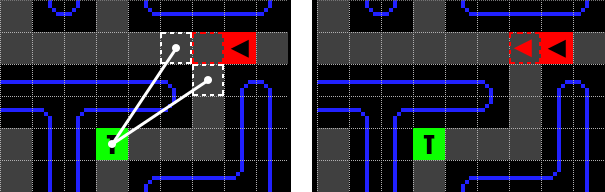
\includegraphics[scale=0.5,]{img/TieBreak.png}
        \caption{Resolución de conflicto de los fantasmas cuando la distancia es la misma. La casilla roja es el fantasma y su dirección y la verde su objetivo. Imagen obtenida de \cite{pittman2015}.}
        \label{fig:decidir}
    \end{center}
\end{figure}

En cuanto al comportamiento individual de cada fantasma entramos en detalle a continuación:

\begin{itemize}
    \item \textbf{Rojo:} es el fantasma que cuenta con un comportamiento más simple, ya que fija como casilla objetivo la posición actual de Pac-Man. Por ello se le considera el fantasma más agresivo de los cuatro. Podemos ver un ejemplo en la figura \ref{fig:red-pink}(a).
    \item \textbf{Rosa:} cuenta con otro comportamiento relativamente simple, ya que fija como casilla objetivo la casilla que se encuentre a cuatro unidades de distancia de la dirección actual de Pac-Man. Esto provoca que este fantasma se dirija generalmente hacia donde se esté moviendo el jugador. Podemos ver un ejemplo en la figura \ref{fig:red-pink}(b).
    \item \textbf{Azul:} utiliza la predicción que usa el fantasma rosa sumado a que traza un segmento cuyo origen es la posición del fantasma rojo, tiene por centro la casilla de la predicción y acaba en la casilla destino. Esto provoca que el fantasma nos encierre y se acerque más cuanto más cerca esté el rojo. Podemos ver un ejemplo en la figura \ref{fig:red-pink}(c).
    
     \begin{figure}[H]
    \centering
        \begin{subfigure}[b]{0.25\textwidth}
            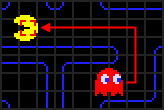
\includegraphics[scale=0.8]{img/red.png}
        \caption{Comportamiento del fantasma rojo.}
        \end{subfigure}
        \hspace{2cm}
        \begin{subfigure}[b]{0.25\textwidth}
            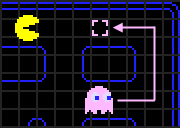
\includegraphics[scale=0.69]{img/pink.png}
            \caption{Comportamiento del fantasma rosa.}
        \end{subfigure}
        \vspace{0.5cm}
        \\
        \begin{subfigure}[b]{0.25\textwidth}
        \centering
            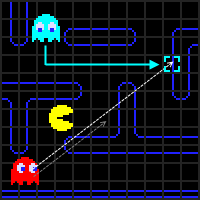
\includegraphics[scale=0.6]{img/blue.png}
            \caption{Comportamiento del fantasma azul.}
        \end{subfigure}
        \caption{Ejemplos de comportamiento de los fantasmas rojo, rosa y azul. Imágenes obtenidas de \cite{druid2016}.}
        \label{fig:red-pink}
    \end{figure}
    
    \item \textbf{Naranja:} quizás es el fantasma con el comportamiento más inofensivo para Pac-Man ya que aunque cuando se encuentra a más de 8 casillas de distancia, se comporta como el fantasma rojo y se dirige a la casilla actual de Pac-Man, cuando entra en ese radio, huye y se comporta similar a cuando se está dispersando.
\end{itemize}

\begin{figure}[H]
    \begin{center}
        \begin{subfigure}[b]{0.49\textwidth}
        \centering
            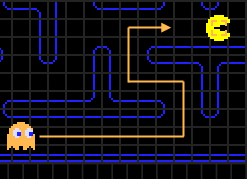
\includegraphics[scale=0.6]{img/orange1.png}
            \caption{Comportamiento de persecución.}
        \end{subfigure}
        \hfill
        \begin{subfigure}[b]{0.49\textwidth}
        \centering
            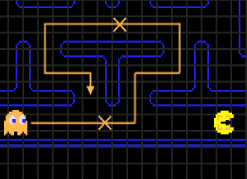
\includegraphics[scale=0.6]{img/orange2.png}
            \caption{Comportamiento de huida.}
        \end{subfigure}
        \caption{Ejemplo de comportamiento del fantasma naranja. Imágenes obtenidas de \cite{druid2016}.}
        \label{fig:blue}
    \end{center}
\end{figure}

% ---------------------------------------------------------------------------- %
\newpage
\subsection{Propuesta}

    El grueso de este proyecto y el objetivo principal del mismo es la aplicación de generación procedimental de contenido \acrshort{pcg} al videojuego clásico Pac-Man. Para ello, se propone aplicar técnicas de \acrshort{pcg} al mapeado, en particular al laberinto, las texturas y la inteligencia artificial del juego.

\subsubsection{Generación de laberintos}

    En particular, implementaremos un algoritmo que genere laberintos para dicho juego. Cuando hablamos de laberintos no solo hablamos de los caminos y muros, sino del nivel al completo del juego, incluyendo otros elementos como por ejemplo los puntos que debe comerse Pac-Man.\\
    
    Siguiendo la clasificación de contenido generado procedimentalmente que hemos establecido en la sección anterior, nuestro problema cae directamente en las categorías de \textit{Game Design}, debido a que los laberintos generados compondrán un nivel del juego, y, principalmente de \textit{Game Systems}, en la subcategoría \textit{Redes de carreteras}. Esto se debe a que nuestro problema no es más que la generación de una serie de caminos en el que se mantiene un equilibrio entre la aleatoriedad de los mismos y una estructura lógica y restricciones en cuanto a la disposición de los elementos que componen el laberinto.\\
    
    Para ello partiremos del método desarrollado en la propuesta e implementación de Shaun LeBron \cite{lebron2012}, creando un modelo y algoritmo propio para la generación procedimental de laberintos del juego Pac-Man.

\subsubsection{Generación de texturas}

    Con el fin de explorar técnicas de generación procedimental de contenido a diversos niveles dentro de la clasificación realizada, se propone explorar la Teselación de Voronoi como método de generación de texturas que aplicaremos a los muros de nuestro escenario.\\
    
    Siguiendo la clasificación de contenido generado procedimentalmente que hemos establecido en la sección anterior, nuestro problema cae directamente en la categoría de \textit{Game Bits}, debido a que las texturas forman parte de las unidades más básicas de contenido que componen un juego.

\subsubsection{Comportamiento de la inteligencia artificial}

    Teniendo en cuenta que el desarrollo de una inteligencia artificial similar a la del juego Pac-Man no es el objetivo de este proyecto, se propone desarrollar una versión simplificada de la misma. Concretamente, se implementará una máquina de estados que defina el comportamiento que deben tomar los fantasmas en cada momento y en lo que a algoritmos de búsqueda de caminos se refiere, utilizaremos el algoritmo de búsqueda A estrella (de ahora en adelante \acrshort{astar}, con su traducción en inglés, \acrlong{astar}).\\
    
    En cuanto a \acrshort{pcg}, alteraremos el comportamiento de los fantasmas mediante parámetros que generaremos procedimentalmente teniendo en cuenta diversos factores como por ejemplo, el nivel actual o la habilidad del jugador. Algunos ejemplos de parámetros que modificarían el comportamiento de los fantasmas sería la agresividad o la persistencia a la hora de perseguir al jugador.
    
    \newpage
    \input{secciones/05_diseño}
    
    \newpage
    \section{Implementación}

En este apartado explicaremos la implementación que se ha llevado a cabo del juego Pacman, haciendo hincapié por una parte en los apartados gráfico y lógico del juego, y por otra centrándonos en cada uno de los apartados en los que se ha aplicado generación procedimental y el método desarrollado para cada caso.

\subsection{Implementación del juego base}

\subsubsection{Apartado gráfico}

Aunque se haya usado una biblioteca gráfica que nos permite cargar modelos \acrshort{3d}, se ha optado por la creación de los modelos tanto de Pac-Man como de los fantasmas a partir de formas geométricas simples. A su vez, se ha usado materiales simples y basados en los del juego original y un fondo negro como en el mismo.\\

Inicialmente, se siguió la misma estética minimalista para la representación gráfica del laberinto y sus componentes, optando por cubos azules y verdes con un borde blanco para los muros y los \textit{`pasillos''} o \textit{`portales''}, y por esferas blancas pequeñas y grandes para los puntos y las \textit{`pastillas''}. Posteriormente, se ha trabajado en la generación procedimental de texturas para los muros del laberinto y en un modelo \acrshort{3d} simple compuesto por un toro y una esfera para los portales.\\

\begin{figure}[H]
    \begin{center}
        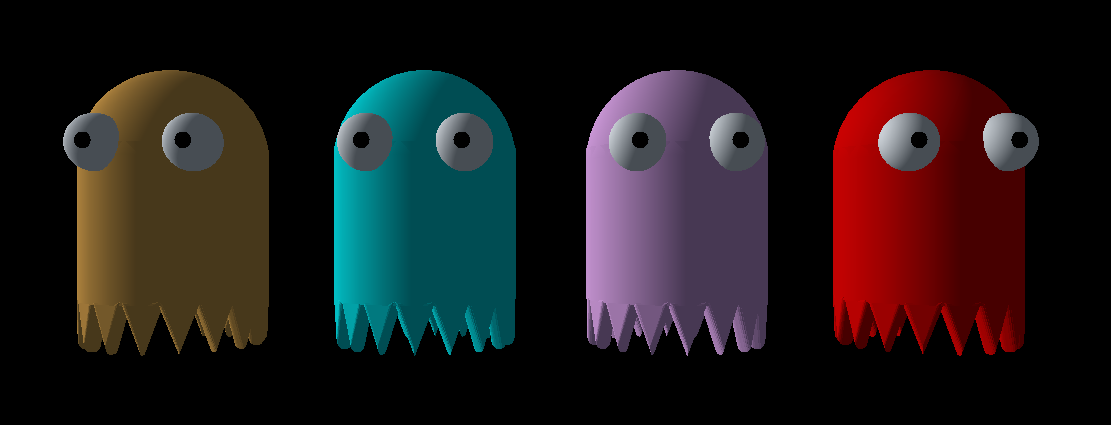
\includegraphics[scale=0.3]{img/fantasmas.png}
        \caption{Modelo \acrshort{3d} de los fantasmas.}
    \end{center}
\end{figure}

En lo que se refiere a las luces, se ha optado por una luz ambiente para evitar se vean negras aquellas zonas donde no incida otra fuente de luz y por una luz focal blanca situada en la parte superior izquierda del escenario.\\

En cuanto a la visualización, se ha creado una cámara en perspectiva, ya que utiliza la proyección en perspectiva que imita al ojo humano, método más utilizado en el renderizado de escenas \acrshort{3d}.

\newpage

\subsubsection{Apartado lógico}

\paragraph{Inteligencia artificial}

Más allá de los factores que modifiquen procedimentalmente el comportamiento de los fantasmas, se ha optado por un algoritmo de búsqueda de caminos \acrshort{astar} básico que utiliza la distancia Manhattan como medida heurística, ya que a efectos prácticos, las distancias que estamos midiendo son las de una cuadrícula y los personajes no cuentan con movimientos en diagonal, teniendo solo que preocuparnos de desplazamientos horizontales y verticales.\\

Por otra parte, los fantasmas cuentan con una máquina de estados que define su comportamiento, definiendo su casilla objetivo en función del estado en el que se encuentren tal y como hacía el juego original.\\

Los estados con los que cuentan son: permanecer en casa, perseguir a Pac-Man, huir de Pac-Man, volver a casa y quedarse quietos. Entre la figura \ref{fig:estados} y la tabla \ref{tab:estados} podemos observar la máquina de estados compuesta por estos cinco estados y las condiciones que deben cumplirse para saltar de un estado a otro.\\

 \begin{figure}[H]
        \begin{center}
            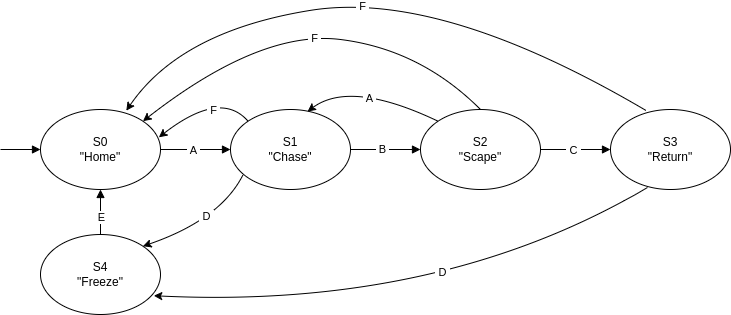
\includegraphics[scale=0.6]{img/estado_fantasmas.png}
            \caption{Máquina de estados que define el comportamiento de los fantasmas.}
            \label{fig:estados}
        \end{center}
    \end{figure}    
    
Aunque en los estados principales de perseguir a Pac-Man e huir de él son similares al juego original, la máquina de estados implementada nos ha permitido controlar en todo momento el comportamiento deseado de los fantasmas, ya que por ejemplo, cuando un fantasma está volviendo a casa solo queremos que se vea afectado por eventos ``radicales'' como que el jugador muera o el jugador supere el nivel actual.

\begin{table}[H]
\centering
    \caption{Condiciones y eventos que provocan un cambio de estado en los fantasmas.}
    \begin{tabular}{|c|l|c|}
    \hline
Variable & Condición                                                                                  & Transición                                                                                        \\ \hline
A        & Ha pasado un tiempo variable                                                               & \begin{tabular}[c]{@{}l@{}}$S0\rightarrow S1$\\ $S2\rightarrow S1$\end{tabular}                     \\\hline
B        & \begin{tabular}[c]{@{}l@{}}Pac-Man se ha comido una\\ píldora de energía\end{tabular}      & $S1\rightarrow S2$                                                                                 \\\hline
C        & \begin{tabular}[c]{@{}l@{}}Pac-Man se ha comido a\\ ese fantasma\end{tabular}              & $S2\rightarrow S3$                                                                                 \\\hline
D        & \begin{tabular}[c]{@{}l@{}}Un fantasma ha atrapado\\ a Pac-Man\end{tabular}                & \begin{tabular}[c]{@{}l@{}}$S1\rightarrow S4$\\ $S3\rightarrow S4$\end{tabular}                     \\\hline
E        & \begin{tabular}[c]{@{}l@{}}Ha terminado la animación \\ de muerte del Pac-Man\end{tabular} & $S4\rightarrow S0$                                                                                 \\\hline
F        & \begin{tabular}[c]{@{}l@{}}Se produce un cambio de\\ nivel\end{tabular}                    & \begin{tabular}[c]{@{}l@{}}$S1\rightarrow S0$\\ $S2\rightarrow S0$\\ $S3\rightarrow S0$\end{tabular} \\\hline
\end{tabular}
\label{tab:estados}
\end{table}

\paragraph{Controles, movimiento y colisiones}

En lo referido al movimiento de los fantasmas y al movimiento y controles de Pac-Man se ha implementado un movimiento lineal, avanzando siempre hacia la dirección hacia la que mira el modelo. Además, esto va acompañado de la posibilidad de girar en las cuatro direcciones para Pac-Man en todo momento y en tres de ellas para los fantasmas, ya que no se les permite realizar giros de 180 grados.\\

En cuanto a las colisiones, se gestionan utilizando cajas de colisión o \textit{hitboxes}. Es un sistema sencillo que nos permite interaccionar tanto con los objetos de nuestro entorno como los muros, los portales o los potenciadores como con los fantasmas.\\

Por último, de cara a mejorar la jugabilidad y manejabilidad del personaje, se han implementado dos mecánicas de movimiento para Pac-Man. En primer lugar, los giros se realizan mediante un buffer que recuerda la última dirección indicada por el jugador y realiza el giro cuando llega a una intersección en la que el movimiento almacenado está permitido. Además este buffer se va actualizando siempre a la última instrucción dada, por lo que facilita la navegabilidad del laberinto. En segundo lugar, se ha implementado un giro ``tardío'' o más permisivo, es decir, que se nos permitirá girar en una intersección incluso si el personaje ha comenzado ya a salir de la misma.\\

Todo esto genera un sistema y unos controles sencillos y permisivos a la vez que precisos, mejorando la experiencia de usuario.

% ---------------------------------------------------------------------------- %

\newpage

\subsection{Generación de laberintos}

En la implementación se han representado los laberintos como una matriz \textit{mazeData}, conteniendo cada una de sus celdas un entero entre 0 y 4 que se traduce en un elemento \textit{MyTile}, formando el mapa final. En el proyecto se han implementado dos métodos, la generación tradicional manual y el grueso de este proyecto, una implementación utilizando generación procedimental.

\begin{table}[H]
    \centering
    \caption{Tipos de baldosas que componen los laberintos.}
    \begin{tabular}{|c|c|c|}
    \hline
    Valor   & Significado & Representación        \\ \hline
    {[}0{]} & Muro        & Cubo azul             \\ \hline
    {[}1{]} & Camino      & Cubo transparente     \\ \hline
    {[}2{]} & Punto       & Esfera blanca pequeña \\ \hline
    {[}3{]} & Pastilla    & Esfera blanca grande  \\ \hline
    {[}4{]} & Portal      & Modelo propio            \\ \hline
    \end{tabular}
\end{table}

\subsubsection{Generación manual}

Es el método estándar basado en laberintos pre-establecidos, no siendo más que la mera representación de nuestro mapeado en la matriz ya citada, introduciendo los datos previamente en nuestro programa. Los laberintos generados manualmente son de tamaño 31x28, tamaño de los mapas originales de Pac-Man. Sin embargo, debido a la sencillez del método, se pueden generar laberintos con otras dimensiones. Aunque sea tan simple, se ha querido hacer mención al mismo ya que ha sido fundamental de cara al desarrollo de la aplicación, permitiendo generar mapas concretos de cara a la realización de pruebas.

\subsubsection{Usando PCG}

El método que se ha desarrollado es una variación basada en la propuesta y explicación de Shaun LeBron \cite{lebron2012}, partiendo de la utilización de piezas de estilo Tetris como propone Lebron pero desarrollando un algoritmo propio para la generación procedimental y aleatoria de laberintos estilo Pac-Man de tamaño 30x30.\\

El método propuesto e implementado se divide principalmente en tres pasos:

\begin{enumerate}
    \item Generación de un modelo simple estilo Tetris.
    \item Conversión a un modelo de caminos.
    \item Creación de otros elementos y modelado final.
\end{enumerate}

En las siguientes secciones describiremos el proceso de generación procedimental de los laberinto y el funcionamiento del algoritmo propio diseñado para tal propósito. Además, en la sección \ref{par:ejemplo} se explicará el proceso mediante imágenes para un caso reducido.

\paragraph{Modelo simple}
Nuestro objetivo es crear una matriz de tamaño 9x5 que rellenaremos de piezas estilo Tetris. Antes de entrar en los detalles del método implementado, debemos definir la representación de las celdas de nuestra matriz y de las consideraciones previas que debemos tener en cuenta para cumplir con los patrones de diseño de niveles establecidos el juego Pac-Man.\\

Como representación de cada celda hemos escogido una tupla de dos elementos que representan si dicha celda tiene borde en su parte superior y en su lateral derecho. Esta representación nos deja cuatro tipos de celdas, la que tiene ambos bordes, la que no tiene ninguno, la que tiene solo el de la derecha y la que tiene solo el de arriba.\\

\begin{figure}[H]
    \begin{center}
        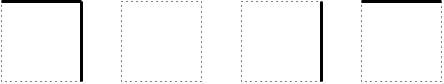
\includegraphics[scale=0.55]{img/celdas.png}
        \caption{Representación de los cuatro tipos de celdas.}
    \end{center}
\end{figure}

Gracias a esta definición, podemos crear un tablero completo de una manera eficiente, ya que los bordes que no definimos en una celda los definen las celdas colindantes. Si guardásemos las cuatro posiciones (arriba, abajo, derecha e izquierda) duplicaríamos la información de los bordes compartidos entre dos piezas.\\

Sin embargo, esta representación no nos permite representar a priori los bordes situados en el lateral izquierdo de las piezas de la primera columna ni los bordes inferiores de las piezas de la última fila, tal y como podemos ver en la figura \ref{fig:representacionColor}.\\

Ambos problemas los solucionaremos más adelante, por lo que por ahora los dejaremos apartados temporalmente. Por otra parte, en la generación de esta matriz 9x5 debemos tener en cuenta que tantos los fantasmas como Pac-Man tienen la misma posición de inicio independientemente del mapa generado, por lo que debemos asegurar que dichas posiciones queden disponibles para los personajes.\\

Por ello aseguraremos, independientemente de la disposición aleatoria de las piezas estilo Tetris, que nuestro modelo simple contendrá las celdas que componen la \textit{``casa''} de los fantasmas (representada por el cuadrado amarillo en la figura \ref{fig:representacionColor}) y que existe un borde en la primera columna, entre la séptima y octava filas, ya que será el punto de aparición de Pac-Man.\\

\begin{figure}[H]
    \centering
        \begin{subfigure}[b]{0.45\textwidth}
            \centering
            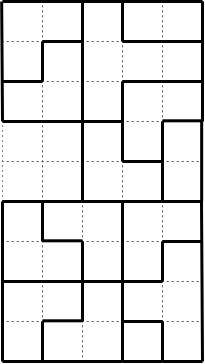
\includegraphics[scale=0.65]{img/grafo.png}
            \caption{Representación simple de los bordes de las piezas.}
        \end{subfigure}
        \hfill
        \begin{subfigure}[b]{0.45\textwidth}
            \centering
            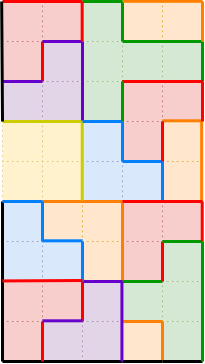
\includegraphics[scale=0.65]{img/grafo_color.png}
            \caption{Representación de los bordes coloreados por piezas.}
        \end{subfigure}
        \caption{Comparación entre los bordes a definir y los definidos utilizando celdas.}
        \label{fig:representacionColor}
\end{figure}


Tomadas estas consideraciones previas, podemos entrar en detalle en qué piezas estilo Tetris usaremos y cómo las añadiremos a nuestra matriz para obtener finalmente el modelo simple. En cuanto a las piezas, definiremos cada pieza como un conjunto de tres-tuplas con N elementos, siendo N el número de cuadrados que compongan la pieza, tuplas que corresponderán a la posición relativa\footnote{El eje Y está invertido debido a que utilizaremos estos valores para recorrer la matriz a la hora de comprobar si la posición de la pieza es válida.} de cada una de las celdas dentro de la pieza (fila, columna) y al tipo de celda que corresponde.\\

\begin{figure}[H]
    \begin{center}
        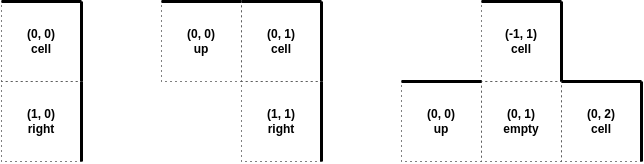
\includegraphics[scale=0.6]{img/piezas.png}
        \caption{Ejemplos de representación de varios tipos de piezas.}
    \end{center}
\end{figure}

A la hora de rellenar nuestra matriz con las piezas, la recorreremos por columnas y seguiremos el siguiente algoritmo de generación por procedimientos:

\begin{enumerate}
    \item Seleccionamos una casilla aleatoria de la columna actual de entre las que no han sido asignadas todavía a una pieza.
    \item Creamos un conjunto de piezas válidas.
    \begin{enumerate}
        \item Seleccionamos una pieza.
        \item Recorremos sus celdas comprobando que su posición relativa respecto a la casilla inicial que seleccionamos se encuentra sin asignar en nuestra matriz.
        \item Repetimos hasta quedarnos sin piezas.
    \end{enumerate}
    \item Seleccionamos una pieza aleatoria del conjunto de piezas válidas\footnote{En el caso de que nos encontrásemos con el conjunto vacío, asignaríamos por defecto una pieza con una única celda con borde en ambos lados.}.
    \item Asignamos los valores de las celdas de la pieza seleccionada a las respectivas posiciones de la matriz.
    \item Repetimos hasta completar la matriz.
\end{enumerate}

Debido a las transformaciones que sufrirá nuestra matriz en la creación del modelo de caminos, en la primera columna hemos definido un conjunto de piezas menor que en el resto. Esta consideración se ha tenido también en la última columna, pero esta vez con el fin de ahorrar comprobaciones innecesarias.\\

Finalmente, antes de pasar al siguiente modelo, solucionaremos el problema de los bordes de la última fila añadiendo una fila a nuestra matriz 9x5 que contenga celdas con únicamente borde superior.

\newpage

\paragraph{Modelo de caminos}

Con el modelo simple creado ahora contamos con una matriz 10x5 que representa los bordes que forman nuestras piezas estilo Tetris.\\

Si observamos nuestro modelo simple, podemos llegar fácilmente a la conclusión que los bordes representados en él no son más que los caminos que formaran nuestro laberinto y que los espacios restantes serán los muros del mismo. Además, también podemos observar que los caminos generados no crean ningún \textit{``callejón sin salida''}, ya que cada nodo del grafo generado cuenta con al menos dos caminos conectados.\\

Ya que nuestro objetivo es crear un laberinto de proporciones similares al laberinto original de Pac-Man de 31x28, si transformamos cada celda de nuestro modelo simple en una nueva de tamaño 3x3, obtendremos una matriz de 30x15. Cada una de nuestras celdas se traducirá convirtiendo los bordes en caminos y los espacios en blanco en muros, tal y como indica la siguiente figura.\\

\begin{figure}[H]
    \begin{center}
        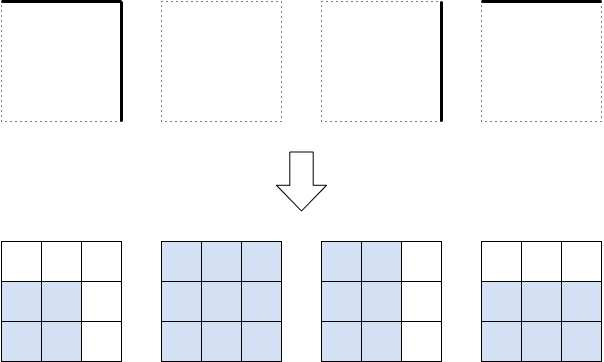
\includegraphics[scale=0.4]{img/celdas3x3.png}
        \caption{Transformación de celdas simples a casillas 3x3.}
    \end{center}
\end{figure}

Aunque las transformaciones propuestas del modelo simple al modelo de caminos implican una traducción casi perfecta de bordes a caminos, se genera una excepción muy específica en la que el modelo no se comporta como debería.\\

Este caso se da cuando encontramos una celda sin bordes con una celda con al menos un borde superior a su derecha y una celda con al menos un borde derecho encima suya. Sin embargo, este caso es fácilmente seleccionable, ya que cuando se de simplemente tendremos que sustituir el valor de la esquina superior derecha de nuestra casilla 3x3 por el de un camino.

\begin{figure}[H]
    \begin{center}
        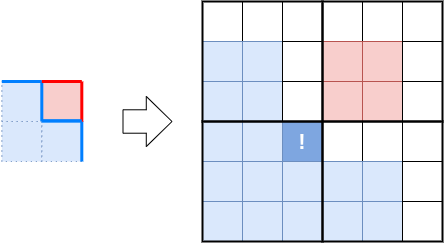
\includegraphics[scale=0.5]{img/grafo3x3.png}
        \caption{Excepción generada por las transformaciones propuestas.}
    \end{center}
\end{figure}

Con esta excepción ya contemplada y con el fin de cumplir con la simetría presente en los laberintos originales del juego, el siguiente paso que debemos dar es el de generar una matriz 30x30 en la que una mitad sea la inversa respecto al eje Y que la otra.\\

Sin embargo, debido a los modelos propuestos y transformaciones realizadas, debemos realizar dos últimos ajustes a nuestro modelo de caminos antes de dar este paso, ya que si se observa detalladamente, el modelo está rodeado de caminos\footnote{Con la excepción del borde inferior, que por el ajuste que hicimos en el modelo simple, ya cuenta con un muro exterior.} mientras que los laberintos deben estar rodeados por muros exteriores.\\

Por ello, actualmente nos faltaría un muro exterior en la primera fila y uno en el lado derecho de nuestro modelo. El primer caso se soluciona con un simple cambio, ya que contamos con dos filas de muro exterior en la parte inferior, desplazando todas las filas una posición hacia abajo y sustituyendo la primera por una de muro.\\

En el segundo caso aprovecharemos para retomar el problema que dejamos pendiente en el modelo simple. Como en el modelo simple no representamos correctamente los bordes de la izquierda de la primera columna, simplemente eliminaremos esa primera columna de nuestro modelo de caminos, dejando espacio para una columna de muro exterior en el extremo derecho de nuestra matriz.\\

Finalmente ya podemos realizar la simetría respecto al eje Y hacia la izquierda, obteniendo una matriz de 30x30 compuesta por caminos y muros.

\newpage
\paragraph{Modelo final}

Con el modelo de caminos terminado, contamos con un laberinto de tamaño 30x30 compuesto de muros y caminos. Por lo tanto, únicamente nos queda dotar a nuestra matriz de los elementos restantes del juego.

\begin{enumerate}
    \item Generación de portales.
    \item Generación de puntos.
    \item Generación de pastillas.
\end{enumerate}

Con el fin de generar más variedad aún de laberintos, se han añadido variantes \textit{``sin camino''} al conjunto de piezas de la última columna, generando posibles \textit{``callejones sin salida''}. Sin embargo, de cara a la generación de portales, supone una gran ventaja, ya que se generan automáticamente posiciones en los que los portales son obligatorios. Aún así, en el caso de no generarse ninguno, generaremos al menos uno de manera aleatoria, escogiendo entre los cruces que se encuentren junto a los muros exteriores laterales.\\

En cuanto a la generación de puntos, rellenaremos todos los caminos disponibles a excepción de una zona segura en el centro del mapa, ya que recoger puntos tan cerca del punto de aparición de los fantasmas no forma parte del juego original. En nuestro caso hemos establecido una zona de 11x14.\\

Finalmente, debemos añadir cuatro pastillas al mapa, aproximadamente en las esquinas del mismo. Para ello, colocaremos a la misma altura las pastillas dos a dos y en la primera y última columna.\\

Con el modelo final ya completo, simplemente traduciremos la matriz de 30x30 generada de manera procedimental a un laberinto formado por elementos del juego, dando como resultado una variedad de mapas prácticamente infinita. Podremos ver varios ejemplos de laberintos generados utilizando nuestro algoritmo en la figura \ref{fig:ejemplos}.\\

     \begin{figure}[H]
    \centering
        \begin{subfigure}[b]{0.48\textwidth}
            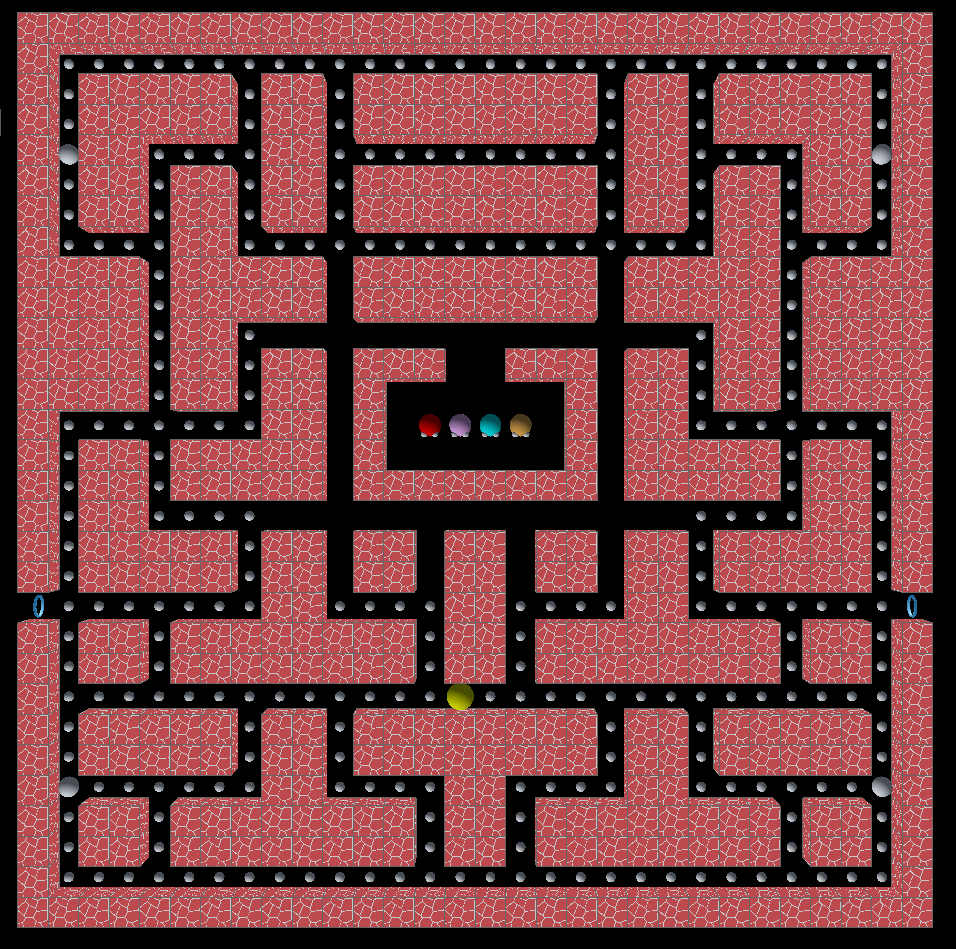
\includegraphics[scale=0.18]{img/laberinto1.png}
        \end{subfigure}
        \hfill
        \begin{subfigure}[b]{0.48\textwidth}
            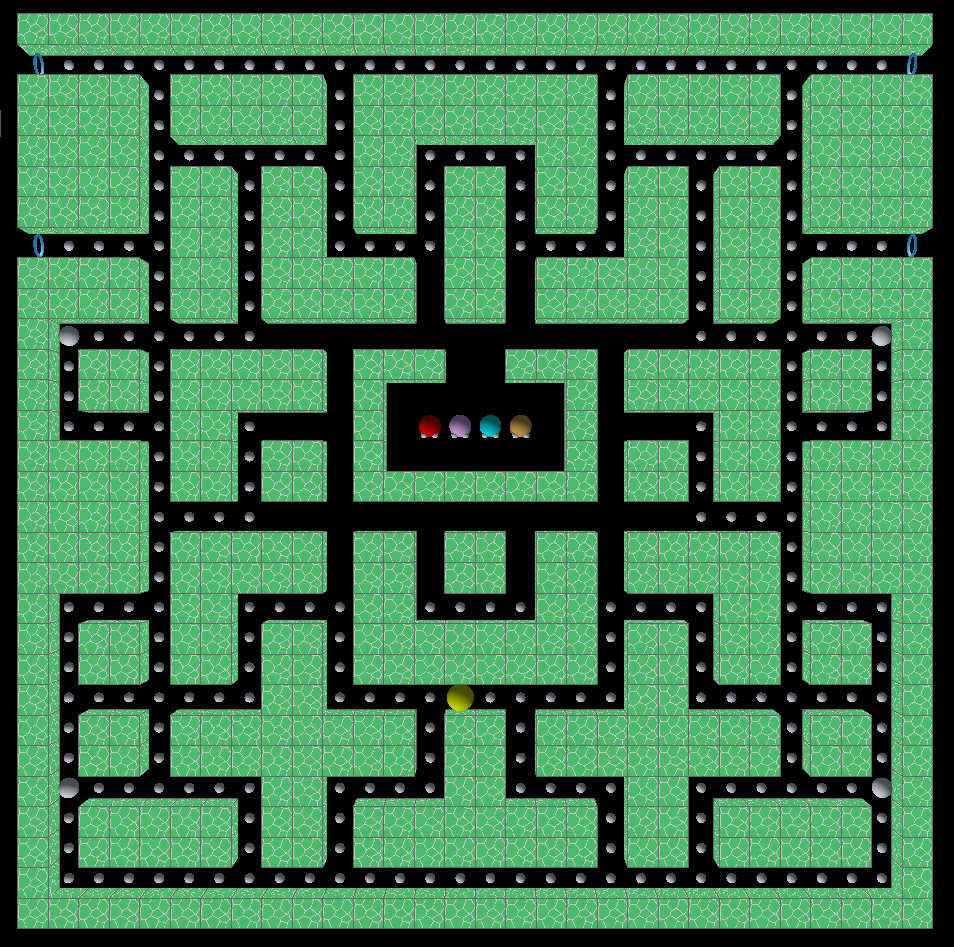
\includegraphics[scale=0.18]{img/laberinto2.png}
        \end{subfigure}
        \vspace{0.2cm}
        \\
        \begin{subfigure}[b]{0.48\textwidth}
            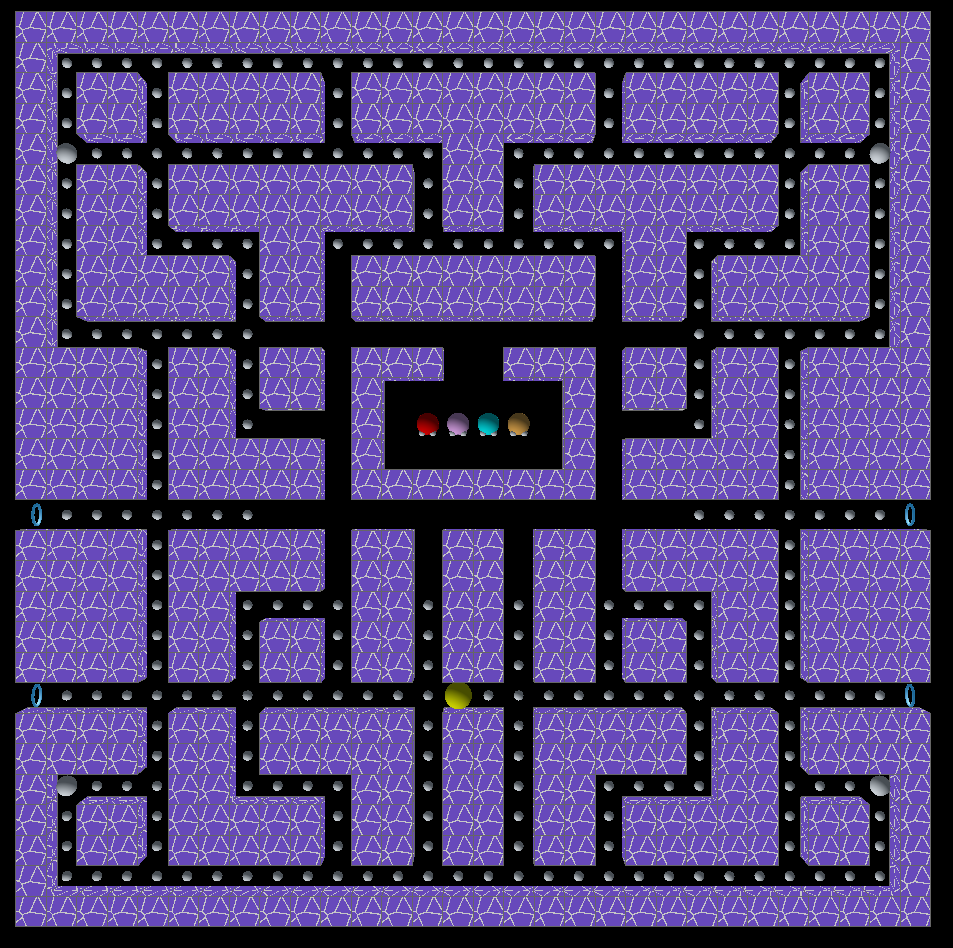
\includegraphics[scale=0.18]{img/laberinto3.png}
        \end{subfigure}
        \hfill
        \begin{subfigure}[b]{0.48\textwidth}
            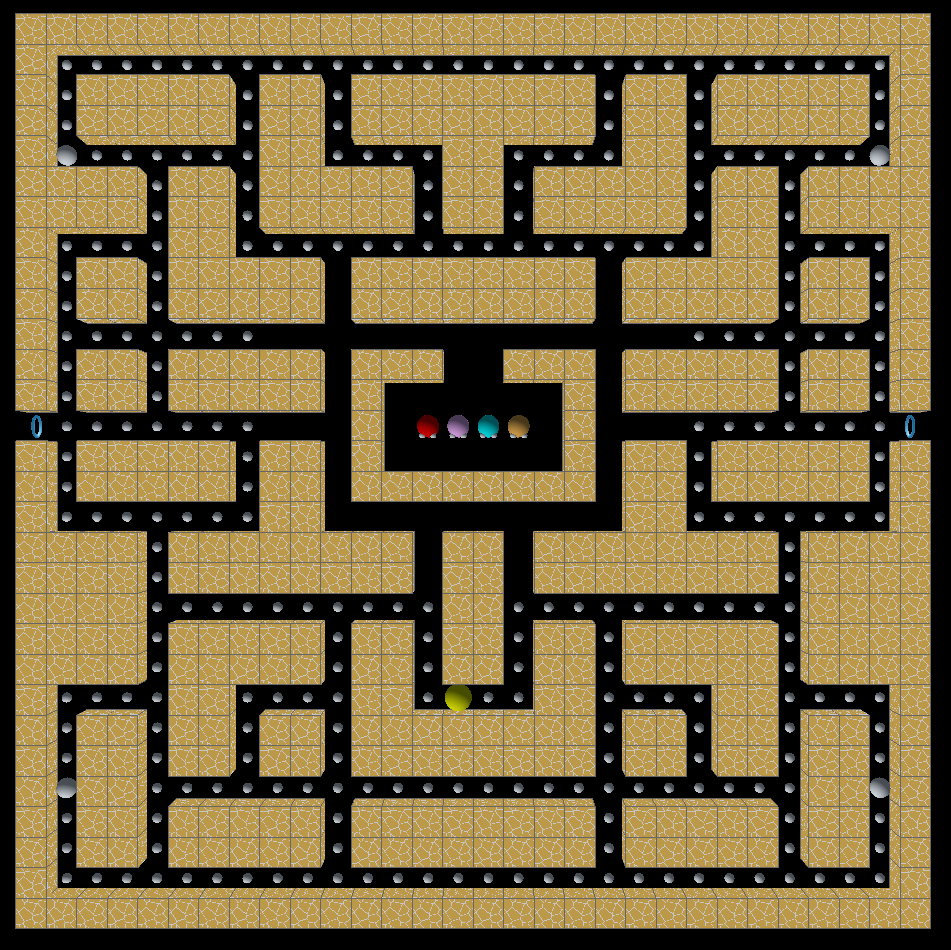
\includegraphics[scale=0.18]{img/laberinto4.png}
        \end{subfigure}
        \vspace{0.2cm}
        \\
        \begin{subfigure}[b]{0.48\textwidth}
            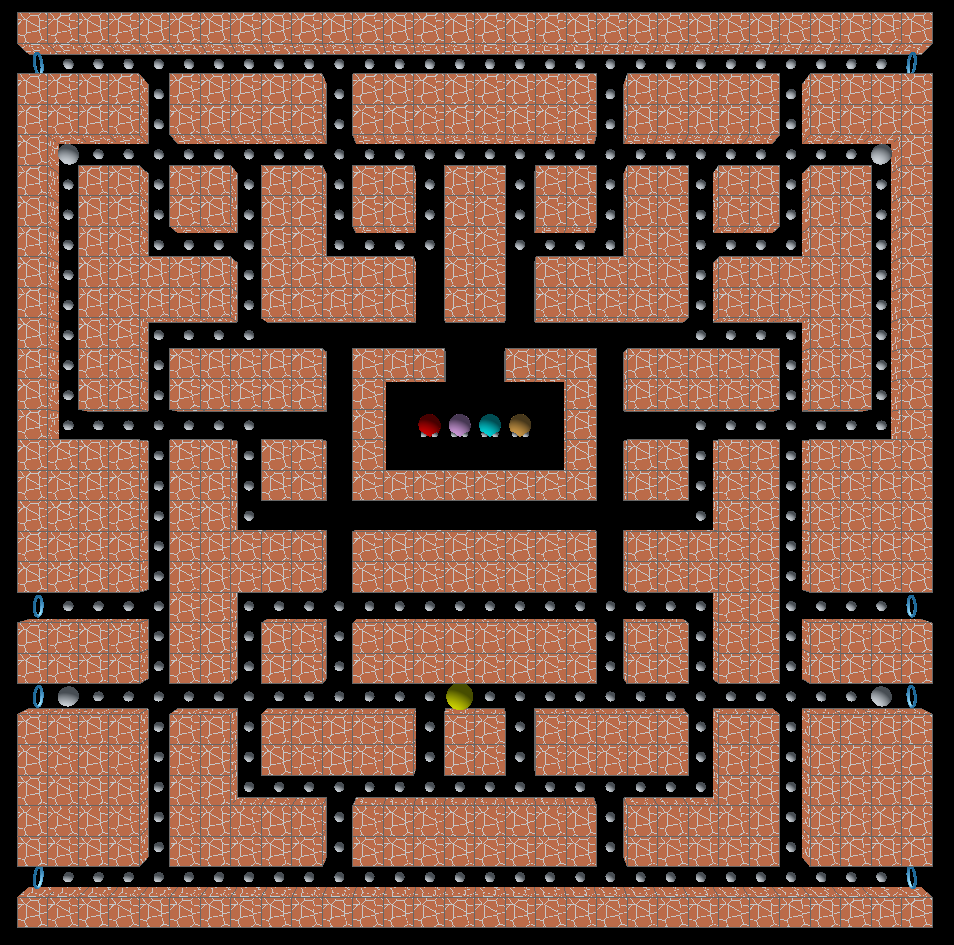
\includegraphics[scale=0.18]{img/laberinto5.png}
        \end{subfigure}
        \hfill
        \begin{subfigure}[b]{0.48\textwidth}
            \includegraphics[scale=0.18]{img/laberinto6.png}
        \end{subfigure}
        \caption{Niveles generados procedimentalmente en la reimplementación de Pac-Man.}
        \label{fig:ejemplos}
    \end{figure}

\paragraph{Ejemplo ilustrado del algoritmo de generación de laberintos}\label{par:ejemplo}

A continuación mostramos un ejemplo paso a paso de la ejecución del algoritmo para un caso reducido de dimensión inicial de 4x4.

    \begin{figure}[H]
    \centering
        \begin{subfigure}[b]{0.9\textwidth}
            \centering
            \includegraphics[scale=0.4]{img/paso1.png}
            \caption{Establecemos los valores de las casillas de la casa de los fantasmas.}
        \end{subfigure}
        \par\bigskip
        \begin{subfigure}[b]{0.9\textwidth}
            \centering
            \includegraphics[scale=0.4]{img/paso2.png}
            \caption{Escogemos una casilla de la primera columna, seleccionamos una pieza de entre el conjunto de piezas válidas y la colocamos en nuestra matriz.}
        \end{subfigure}
        \par\bigskip
        \begin{subfigure}[b]{0.9\textwidth}
            \centering
            \includegraphics[scale=0.4]{img/paso3.png}
            \caption{Escogemos la única casilla restante de la primera columna. Al ir a seleccionar una pieza y estar vacío el conjunto de piezas válidas, rellenamos la casilla por defecto con una celda completa.}
        \end{subfigure}
        \caption{Ejemplo ilustrado del algoritmo de generación de laberintos - Modelo simple.}
        \label{fig:simple1}
    \end{figure}
    
    \begin{figure}[H]
    \ContinuedFloat 
    \centering
        \begin{subfigure}[b]{0.95\textwidth}
            \centering
            \includegraphics[scale=0.45]{img/paso4.png}
            \caption{Cambiamos a la tercera columna ya que la segunda ya está completa. Escogemos una casilla de la columna, seleccionamos una pieza entre las piezas válidas y la colocamos en nuestra matriz.}
        \end{subfigure}
        \par\bigskip
        \begin{subfigure}[b]{0.95\textwidth}
            \centering
            \includegraphics[scale=0.45]{img/paso5.png}
            \caption{Volvemos a repetir el paso anterior. Escogemos una casilla de la columna, seleccionamos una pieza entre las piezas válidas y la colocamos en nuestra matriz.}
        \end{subfigure}
        \par\bigskip
        \begin{subfigure}[b]{0.95\textwidth}
            \centering
            \includegraphics[scale=0.45]{img/paso6.png}
            \caption{Escogemos la única casilla restante de la tercera columna. Al ir a seleccionar una pieza y estar vacío el conjunto de piezas válidas, rellenamos la casilla por defecto con una celda completa.}
        \end{subfigure}
        \caption{Ejemplo ilustrado del algoritmo de generación de laberintos - Modelo simple.}
        \label{fig:simple2}
    \end{figure}
    
    \begin{figure}[H]
    \ContinuedFloat 
    \centering
        \begin{subfigure}[b]{0.95\textwidth}
            \centering
            \includegraphics[scale=0.45]{img/paso7.png}
            \caption{Cambiamos a la cuarta columna y escogemos la única casilla restante. Al estar vacío el conjunto de piezas válidas, rellenamos la casilla por defecto con una celda completa.}
        \end{subfigure}
        \par\bigskip
        \begin{subfigure}[b]{0.95\textwidth}
            \centering
            \includegraphics[scale=0.45]{img/paso8.png}
            \caption{Hemos terminado de rellenar la matriz 4x4 que forma el modelo simple.}
        \end{subfigure}
        \par\bigskip
        \begin{subfigure}[b]{0.95\textwidth}
            \centering
            \includegraphics[scale=0.45]{img/paso9.png}
            \caption{Antes de avanzar al modelo de caminos, añadiremos una fila de celdas con borde superior en la parte inferior de nuestra matriz.}
        \end{subfigure}
        \caption{Ejemplo ilustrado del algoritmo de generación de laberintos - Modelo simple.}
        \label{fig:simple3}
    \end{figure}
% ---------------------------------------------------------------------------- %

    \begin{figure}[H]
    \centering
        \begin{subfigure}[b]{0.95\textwidth}
            \centering
            \includegraphics[scale=0.375]{img/paso10.png}
            \caption{Transformamos el modelo simple aplicando las equivalencias de celdas simples a casillas 3x3, dando como resultado una nueva matriz de tamaño 15x12.}
        \end{subfigure}
        \par\bigskip
        \begin{subfigure}[b]{0.45\textwidth}
            \centering
            \includegraphics[scale=0.375]{img/paso11.png}
            \caption{Eliminamos la primera columna y la última fila de la matriz resultante. Además, añadimos una fila al principio y una columna al final compuestas exclusivamente de muro.}
        \end{subfigure}
        \hfill\begin{subfigure}[b]{0.45\textwidth}
            \centering
            \includegraphics[scale=0.375]{img/paso12.png}
            \caption{Con estas transformaciones y modificaciones hemos completado el modelo de caminos, obteniendo una matriz de tamaño 15x12 compuesta por caminos y muros.}
        \end{subfigure}
        \caption{Ejemplo ilustrado del algoritmo de generación de laberintos - Modelo de caminos.}
        \label{fig:caminos}
    \end{figure}
% ---------------------------------------------------------------------------- %

    \begin{figure}[H]
    \centering
    \begin{subfigure}[b]{0.95\textwidth}
            \centering
            \includegraphics[scale=0.45]{img/paso13.png}
            \caption{Realizamos la simetría respecto al eje Y hacia la izquierda, obteniendo una matriz de 30x15 que forma un laberinto cerrado y válido.}
        \end{subfigure}
        \par\bigskip
        \begin{subfigure}[b]{0.95\textwidth}
            \centering
            \includegraphics[scale=0.45]{img/paso14.png}
            \caption{Realizamos modificaciones para añadir o quitar muros, como por ejemplo, eliminamos los muros de la zona de la casa de los fantasmas.}
        \end{subfigure}
        
        \par\bigskip
        \begin{subfigure}[b]{0.95\textwidth}
            \centering
            \includegraphics[scale=0.45]{img/paso15.png}
            \caption{En el caso de que no se hayan generado callejones sin salida, seleccionamos los posibles candidatos para la generación de portales, asegurando así que habrá al menos un portal.}
        \end{subfigure}
        \caption{Ejemplo ilustrado del algoritmo de generación de laberintos - Modelo final.}
        \label{fig:final1}
        
    \end{figure}
    
    \begin{figure}[H]
    \ContinuedFloat 
    \centering
    \begin{subfigure}[b]{0.95\textwidth}
            \centering
            \includegraphics[scale=0.45]{img/paso16.png}
            \caption{Colocamos los puntos dejando una zona libre alrededor de la casa de los fantasmas. Añadimos los potenciadores o pastillas en las cuatro esquinas del mapa.}
        \end{subfigure}
        \par\bigskip
        \begin{subfigure}[b]{0.95\textwidth}
            \centering
            \includegraphics[scale=0.45]{img/paso17.png}
            \caption{Con ello ya dispondríamos de una matriz \textit{MazeData} compuesta por muros, caminos, puntos, pastillas y portales, y que podremos traducir a un nivel generado procedimentalmente del juego \textit{Pac-Man}.}
        \end{subfigure}
        
        \caption{Ejemplo ilustrado del algoritmo de generación de laberintos - Modelo final.}
        \label{fig:final2}
    \end{figure}
% ---------------------------------------------------------------------------- %

\newpage

\subsection{Generación de texturas}

En la implementación se ha trabajado con un shader utilizando el tipo de material \textit{ShaderMaterial} proporcionado por la biblioteca Three.js y partiendo de la implementación de Iñigo Quílez \cite{quilez} de las distancias de Voronoi.\\

Para conseguir lograr variedad de patrones y reducir lo máximo posible las repeticiones o texturas muy similares, hemos jugado con tres factores que afectan a la generación de los patrones de Voronoi. En primer lugar modificamos cada vez que se crea la textura los dos vectores en los que se basa el algoritmo. En segundo lugar variamos la granularidad o cantidad de celdas del patrón, generando patrones con celdas de mayor a menor tamaño. Por último y con el fin de añadir aún más variedad de texturas, modificamos el valor del \textit{Hue} o tonalidad del color.

\begin{table}[H]
    \centering
    \caption{Variables y rango de valores que modifican la textura.}
    \begin{tabular}{|l|l|l|}
    \hline
    Variable & Rango de valores                                                         & Consecuencia                     \\ \hline
    vecA     & \begin{tabular}[c]{@{}l@{}}{[}75.0,150.0)\\ {[}200.0,350.0)\end{tabular} & Modifica el patrón               \\ \hline
    vecB     & \begin{tabular}[c]{@{}l@{}}{[}75.0,150.0)\\ {[}200.0,350.0)\end{tabular} & Modifica el patrón               \\ \hline
    amount   & {[}0.25, 0.5)                                                            & Modifica el tamaño de las celdas \\ \hline
    Hue      & {[}0.0, 1.0)                                                             & Modifica el color                \\ \hline
    \end{tabular}
\end{table}

Estas modificaciones se ejecutan cada vez que generamos un laberinto nuevo, aportando aún más variedad de la ya conseguida con la generación de laberintos implementada en la sección anterior.\\

\begin{figure}[H]
    \begin{center}
        \includegraphics[scale=0.275]{img/texturas.png}
        \caption{Ejemplos de variedad de texturas generadas procedimentalmente usando Teselación de Voronoi.}
    \end{center}
\end{figure}

% ---------------------------------------------------------------------------- %

\newpage

\subsection{Comportamiento de la inteligencia artificial}

Con el fin de generar una dificultad adaptativa a la habilidad del jugador y progresiva según avance la partida, modificaremos tres variables relacionadas con el comportamiento de los fantasmas: tiempo de espera en casa, tiempo que permanecen asustados y que pueden ser comidos por Pac-Man y frecuencia con la que actualizan el camino que están siguiendo.\\

En primer lugar, al reducir el tiempo de espera en casa reducimos la ventana de tiempo en la que el jugador solo tiene que preocuparse por un menor número de enemigos que le persigan.\\

En segundo lugar, al reducir el tiempo que permanecen asustados los fantasmas, reducimos la ventana de tiempo en la que el personaje es invencible y no tiene porqué preocuparse de huir de los enemigos.\\

Por último, al aumentar la frecuencia con la que los fantasmas calculan un nuevo camino hasta la posición de Pac-Man provoca que los fantasmas sean más agresivos y precisos a la hora de localizar al personaje. Podemos ver un resumen de las consecuencias de estas modificaciones del comportamiento y el decremento que se le aplica por nivel a cada variable en la tabla \ref{tab:comportamiento}.\\

\begin{table}[H]
\centering
    \caption{Valores que modifican directa e indirectamente el comportamiento de los fantasmas y generan una dificultad progresiva.}
    
\begin{tabular}{|l|l|l|l|l|}
\hline
Variable                                                         & \begin{tabular}[c]{@{}l@{}}Valor\\ inicial\end{tabular} & \begin{tabular}[c]{@{}l@{}}Decremento\\ por nivel\end{tabular} & \begin{tabular}[c]{@{}l@{}}Valor\\ mínimo\end{tabular} & Efecto                                                                                                                     \\ \hline
\begin{tabular}[c]{@{}l@{}}Tiempo\\ en casa\end{tabular}         & 5s                                                      & 0.1s                                                           & 3s                                                     & \begin{tabular}[c]{@{}l@{}}Menos tiempo sin los cuatro\\ fantasmas en pantalla\end{tabular}                                \\ \hline
\begin{tabular}[c]{@{}l@{}}Tiempo\\ asustado\end{tabular}        & \begin{tabular}[c]{@{}l@{}}10s\\ +5s\end{tabular}       & 0.5s                                                           & \begin{tabular}[c]{@{}l@{}}0.1s\\ +5s\end{tabular}     & \begin{tabular}[c]{@{}l@{}}Menor ventana de tiempo para\\ eliminar a los enemigos\end{tabular}                             \\ \hline
\begin{tabular}[c]{@{}l@{}}Tiempo\\ entre\\ caminos\end{tabular} & 7.5s                                                    & 0.2s                                                           & 2s                                                     & \begin{tabular}[c]{@{}l@{}}Mayor agresividad y precisión\\ de los enemigos a la hora de\\ localizar a Pac-Man\end{tabular} \\ \hline
\end{tabular}
\label{tab:comportamiento}
\end{table}
    
    % Conclusiones
    \newpage
    \section{Conclusiones y trabajos futuros}

Para terminar esta memoria haremos un reflexión en lo que se refiere a generación procedimental de contenido en el ámbito de los videojuegos como al aprendizaje realizado y conocimiento adquirido durante el desarrollo de este proyecto. Además, valoraremos los resultados obtenidos fruto de este proyecto, haciendo especial hincapié en lo logrado al aplicar generación procedimental a un videojuego clásico.\\

En primer lugar debemos hablar obligatoriamente del conocimiento adquirido a lo largo del desarrollo de este proyecto, partiendo de no conocer la generación procedimental de contenidos más allá de ser un concepto lejano y difuso, y llegando a tras estas 30 semanas, haber leído multitud de artículos e información relacionada con generación procedimental; haber entrado de lleno en su uso en el sector de los videojuegos, siendo capaz de establecer una clasificación del contenido generado, de los métodos empleados y de las propiedades deseables en estos. Todo ello culminando en la aplicación de técnicas de generación procedimental a un videojuego clásico como el escogido, Pac-Man.\\

Ya entrando en el proyecto específico, se ha logrado una reproducción fiel del videojuego escogido, aportando un enfoque personal y adaptándolo a un entorno en el que la responsabilidad recae principalmente en el programador y que ha permitido precisamente afrontar los conflictos propios de un entorno a más bajo nivel que el que puede proporcionar un motor de videojuegos. Precisamente la elección de Three.js para el desarrollo de este proyecto me ha permitido seguir fortaleciendo conocimientos adquiridos durante los estudios de Grado, algunos tan imprescindibles como puede ser la importancia de una gestión adecuada de la memoria.\\

Todo esto ha servido como base para desarrollar un algoritmo de generación procedimental de laberintos para el videojuego Pac-Man y que ha sido complementado con la generación procedimental de texturas para los muros de los laberintos y una mejora progresiva de la dificultad intrínseca a los comportamientos de la inteligencia artificial. Debemos destacar que las técnicas aplicadas caen directamente en la categoría de métodos tradicionales y generan contenido de varios niveles de la clasificación establecida, como son las texturas que pertenecen a los \textit{Game Bits} o los laberintos y el escenario que pertenecen al \textit{Game Space} y los \textit{Game Scenarios} relativamente.\\

En concreto para la generación de laberintos se ha diseñado un algoritmo que cumple prácticamente con la totalidad de las propiedades deseables para métodos de generación procedimental de contenido. El algoritmo genera niveles del juego en décimas de segundo, el contenido generado es de calidad ya que siempre genera laberintos válidos y jugables, sumado a la inclusión de las texturas, ofrece una variedad casi infinita de mapas distintos, siendo además ampliable y escalable simplemente añadiendo un mayor número de piezas estilo Tetris al conjunto utilizado, y finalmente, todo este contenido imita con facilidad el contenido generado por humanos, ofreciendo credibilidad.\\

Aún con estos logros, el proyecto ha abierto las puertas a otros tantos retos e inquietudes que perseguir en el futuro, tanto a nivel de mejora del propio proyecto software como a nivel de continuar el aprendizaje sobre generación procedimental.\\ 

Por una parte y respecto al proyecto podríamos destacar la mejora a nivel de aplicación, evolucionando de una herramienta cuyo propósito principal es mostrar las posibilidades que nos abre la generación procedimental de contenido a un videojuego propiamente dicho, con menús de opciones, una mejor progresión de dificultad o una inteligencia artificial aún más pulida.\\

Por otra parte, el proyecto no ha hecho más que abrirme los ojos ante el mundo de posibilidades que ofrece la generación procedimental de contenido. Por un lado, sería interesante explorar la posibilidad de combinar el algoritmo diseñado con métodos basados en búsqueda, permitiendo no solo crear infinidad de laberintos sino también clasificar y puntuar los mismos, permitiendo utilizar laberintos más sencillos en los primeros niveles e ir escalando la dificultad en lo que a distribución del escenario se refiere. Por otro lado, me planteo como proyecto futuro seguir investigando y aprendiendo sobre generación procedimental de contenido y en particular me propongo como objetivo próximo aprender sobre el algoritmo de colapso de la función de onda, ya que me ha resultado fascinante los resultados que produce.\\

Concluyamos remarcando el potencial que representa la generación procedimental de contenidos en el ámbito de los videojuegos, no solo permitiéndonos crear una cantidad prácticamente infinita de contenido de calidad sino que nos aporta un nuevo enfoque de cara al desarrollo y diseño de videojuegos.
    
    % Referencias
    \newpage
    \section{Referencias}

\begin{thebibliography}{1}

    %--------- #A ---------%

    \bibitem[Amato, 2017]{amato2017}
	
	\href{https://doi.org/10.1007/978-3-319-53088-8_2}{Amato, A. (2017). Procedural content generation in the game industry. En O. Korn \& N. Lee (Eds.), Game Dynamics (pp. 15-25). Springer International Publishing.}

    %--------- #B ---------%

    \bibitem[Bandai Namco, 2021]{officialSitePacman}
	
	\href{https://pacman.com/en/history/}{BANDAI NAMCO Entertainment Inc. (2021). History - The Official Site for PAC-MAN.}
	
	\bibitem[Barriga, 2019]{barriga2019}
	
	\href{https://doi.org/10.1142/S0218213019300011}{Barriga, N. A. (2019). A short introduction to procedural content generation algorithms for videogames. International Journal on Artificial Intelligence Tools, 28(02), 1930001.}
	
	\bibitem[Blizzard Entertainment, 2000]{diablo}
	
	\href{https://web.archive.org/web/20000815065620/http://www.blizzard.com/diablo/}{Blizzard Entertainment. (2000). Diablo.}
	
	\bibitem[BossladyB, 2020]{eliteDangerous}
	
	\href{https://www.reddit.com/r/EliteDangerousPics/comments/ezqji1/it_was_worth_the_detour/}{BossladyB. (2020). It was worth the detour!}
	
	\bibitem[Braben \& Bell, 2007]{braben2007}
	
	\href{https://web.archive.org/web/20100127094607/http://frontier.co.uk/games/elite}{Braben, D., \& Bell, I. (2007). Games by Frontier Developments.}
	
	\bibitem[Breda University, 2021]{EP}
	
	\href{http://everythingprocedural.com/}{Breda University of Applied Sciences. (2021). EPC2021—Everything Procedural Conference.}
	
	%--------- #C ---------%
	
	\bibitem[Cabello, s.f.-a]{githubThree}
	
	\href{https://github.com/mrdoob/three.js}{Cabello, R. ``Mr.doob'' (s.f.). Github - Three.js.}
	
	\bibitem[Cabello, s.f.-b]{three.js}
	
	\href{https://threejs.org/}{Cabello, R. ``Mr.doob'' (2021). Three.js – JavaScript 3D Library.}
	
	\bibitem[Chirinea, 2008]{chirinea}
	
	\href{https://www.mobygames.com/game/windows/kkrieger-chapter-1/screenshots/gameShotId,280133/}{Chirinea. (2008). Kkrieger: Chapter 1 Screenshots for Windows. En MobyGames.}
	
    \bibitem[Collins, 2017]{collins2017}
	
	\href{https://medium.com/@homicidalnacho/a-look-into-procedural-generation-dfa62fe7536d}{Collins, T. (2017). A look into procedural generation. Medium.}
	
	%--------- #D ---------%
	
	\bibitem[Dinosaur Polo Club, 2019]{dinosaurPolo}
	
	\href{https://store.steampowered.com/app/1127500/Mini_Motorways/}{Dinosaur Polo Club. (2019). Mini Motorways. En Steam.}
	
	%--------- #E ---------%
	
	\bibitem[Edwards, 2011]{edwards2011}
	
	\href{https://doi.org/10.1145/1965724.1965742}{Edwards, M. (2011). Algorithmic composition: computational thinking in music. Communications of the ACM, 54(7), 58-67.}
	
	\bibitem[Electronic Arts, s. f.]{spore}
	
	\href{https://www.ea.com/es-es/games/spore/spore}{Electronic Arts. (s. f.). Spore.}
	
	\bibitem[Eno, 1996]{eno1996}
	
	\href{https://inmotionmagazine.com/eno1.html}{Eno, B. (1996). A talk delivered in San Francisco. In Motion Magazine.}
	
	\bibitem[Epyx Inc., 1985]{epyx}
	
	\href{https://store.steampowered.com/app/1443430/Rogue/}{Epyx Inc. (1985). Rogue. En Steam.}
	
	%--------- #G ---------%
	
	\bibitem[Glenn Stevens, 2021]{glenn2021}
	
	\href{https://www.thegamer.com/best-procedurally-generated-games-minecraft/}{Glenn Stevens, R. (2021, abril 12). The 10 best procedurally-generated games that aren’t minecraft. En TheGamer.}
	
	\bibitem[Grendel Games, s. f.]{grendel-games}
	
	\href{https://grendelgames.com/procedural-generation/}{Grendel Games. (s. f.). Procedural generation.}
	
	%--------- #H ---------%
	
	\bibitem[Hello Games, s. f.]{nomansky}
	
	\href{https://www.nomanssky.com/}{Hello Games. (s. f.). No Man’s Sky.}
	
	\bibitem[Hendrikx et al., 2013]{hendrikx2013}
	
	\href{https://doi.org/10.1145/2422956.2422957}{Hendrikx, M., Meijer, S., Van Der Velden, J., \& Iosup, A. (2013). Procedural content generation for games: A survey. ACM Transactions on Multimedia Computing, Communications, and Applications, 9(1), 1-22.}
	
	%--------- #I---------%
	
	\bibitem[Interactive Data Visualization, s. f.]{speedtree}
	
	\href{https://store.speedtree.com/games/}{Interactive Data Visualization. (s. f.). SpeedTree for Games.}
	
	%--------- #J---------%
	
	\bibitem[Jain et al., 2016]{jain2016}
	
	\href{http://julian.togelius.com/Jain2016Autoencoders.pdf}{Jain, R., Isaksen, A., Holmgård, C., \& Togelius, J. (2016). Autoencoders for level generation, repair, and recognition. In Proceedings of the ICCC workshop on computational creativity and games (p. 9).}
	
	\bibitem[JakePhoenix, 2016]{jake}
	
	\href{https://imgur.com/gallery/XlGEy}{JakePhoenix. (2016). A jungle moon. En Imgur.}
	
	%--------- #K---------%
	
	\bibitem[Kaitila, 2017]{kaitila2017}
	
	\href{https://www.procjam.com/tutorials/en/music/}{Kaitila, C. ``McFunkypants'' (2017). Procedural music generation. PROCJAM 2017.}

    \bibitem[(Khan Academy, s. f.)]{perlin}
	
	\href{https://www.khanacademy.org/computing/computer-programming/programming-natural-simulations/programming-noise/a/perlin-noise}{Khan Academy. (s. f.). Perlin Noise.}
	
	\bibitem[Kim, 2016]{kim2016}
	
	\href{https://doi.org/10.3390/sym8090093}{Kim, J. (2016). Modeling and optimization of a tree based on virtual reality for immersive virtual landscape generation. Symmetry, 8(9), 93.}
	
	\bibitem[Kosh, 2007]{kosh}
	
	\href{https://www.scenebeta.com/noticia/kkrieger}{Kosh. (2007). KKrieger.}
	
	%--------- #L---------%
	
	\bibitem[LeBron, 2012]{lebron2012}
	
    \href{https://shaunlebron.github.io/pacman-mazegen/}{LeBron, S. (2012). Pac-Man Maze Generation.}
	
	\bibitem[Logos, s.f.]{dungeonTiles}
	
	\href{http://dysonlogos.blog/}{Logos, D. (s.f.). Dyson’s Dodecahedron.}
	
	%--------- #M ---------%
	
	\bibitem[Manocha et al., 2009]{manocha2009}
	
	\href{https://doi.org/10.1145/1667239.1667254}{Manocha, D., Calamia, P., Lin, M. C., Savioja, L., \& Tsingos, N. (2009). Interactive sound rendering. ACM SIGGRAPH Courses (SIGGRAPH’09). ACM, New York, 1–338.}
	
	\bibitem[Massive Software, s.f.]{massive}
	
	\href{http://massivesoftware.com/}{Massive Software. (s.f.). Massive – simulating life.}
	
	\bibitem[Microsoft, s.f.-a]{githubPages}
	
	\href{https://pages.github.com/}{Microsoft Corporation. (s. f.-a). Github Pages.}
	
	\bibitem[Microsoft, s.f.-b]{github}
	
	\href{https://github.com/}{Microsoft Corporation. (s.f.). GitHub: Where the world builds software.}
	
	\bibitem[Molina et al., 2020]{molina2020}
	
	\href{https://doi.org/10.1109/TCIAIG.2011.2148116}{Molina, D., Poyatos, J., Ser, J. D., García, S., Hussain, A., \& Herrera, F. (2020). Comprehensive taxonomies of nature- and bio-inspired optimization: Inspiration versus algorithmic behavior, critical analysis recommendations. Cognitive Computation, 12(5), 897-939.}
	
	%--------- #N ---------%
	
	\bibitem[Night Druid, 2016]{druid2016}
	
	\href{https://steamcommunity.com/sharedfiles/filedetails/?id=593226813}{Night Druid. (2016). Pac-Man—Guide to Mastering the Maze!}
	
	%--------- #P ---------%
	
	\bibitem[Pittman, 2015]{pittman2015}
	
	\href{https://pacman.holenet.info/}{Pittman, J. (2015). The Pac-Man Dossier.}
	
	%--------- #Q ---------%
	
	\bibitem[Quílez, 2013]{quilez}
	
	\href{https://www.iquilezles.org/www/articles/voronoilines/voronoilines.htm}{Quílez, I. (2013). Shader example—Voronoi with borders.}
	
	%--------- #R ---------%
	
	\bibitem[Red Hook Studios, 2015]{redhook}
	
	\href{https://store.steampowered.com/app/262060/Darkest_Dungeon/}{Red Hook Studios. (2015). Darkest Dungeon. En Steam.}
	
	%--------- #S ---------%
	
	\bibitem[Shaker et al., 2016]{shaker2016}
	
	\href{https://doi.org/10.1007/978-3-319-42716-4}{Shaker, N., Togelius, J., \& Nelson, M. J. (2016). Procedural content generation in games. Springer International Publishing.}
	
	\bibitem[Smith, 2014]{smith2014}
	
	\href{https://doi.org/10.1145/2556288.2557341}{Smith, G. (2014). Understanding procedural content generation: a design-centric analysis of the role of PCG in games.  In Proceedings of the SIGCHI Conference on Human Factors in Computing Systems, 917-926.}
	
	\bibitem[Smith, 2015]{smith2015}
	
	\href{http://sokath.com/home/wp-content/uploads/2018/01/smith-fdg15.pdf}{Smith, G. (2015). An Analog History of Procedural Content Generation. In Foundations of Digital Games.}
	
	\bibitem[Snodgrass \& Ontañón, 2017]{snodgrass2017}
	
	\href{https://doi.org/10.1109/TCIAIG.2016.2623560}{Snodgrass, S., \& Ontañón, S. (2017). Learning to generate video game maps using Markov models. IEEE Transactions on Computational Intelligence and AI in Games, 9(4), 410-422.}
	
	\bibitem[SoylentGreen, 2007]{voronoi2007}
	
	\href{https://commons.wikimedia.org/wiki/File:Blender3D_VoronoiCrackle.jpg}{SoylentGreen. (2007). Blender3D Voronoi Crackle. En Wikipedia.}
	
	\bibitem[Sportelli et al., 2014]{sportelli2014}
	
	\href{https://doi.org/10.13140/2.1.3820.4163}{Sportelli, F., Toto, G., \& Vessio, G. (2014). A probabilistic grammar for procedural content generation.}
	
	\bibitem[Stålberg, 2020]{oscar}
	
	\href{https://store.steampowered.com/app/1291340/Townscaper/}{Stålberg, O. (2020). Townscaper. En Steam.}
	
	\bibitem[Strandgaard, 2008a]{redPerlin}
	
	\href{https://www.flickr.com/photos/12739382@N04/2415197699/}{Strandgaard, S. (2008a). Pink/red liquid using perlin noise + bump + coloring.}
	
	\bibitem[Strandgaard, 2008b]{lavaPerlin}
	
	\href{https://www.flickr.com/photos/12739382@N04/2630483563/}{Strandgaard, S. (2008b). Perlin noise with bump.}
	
	\bibitem[Strandgaard, 2009]{camuflajePerlin}
	
	\href{https://www.flickr.com/photos/12739382@N04/3628571124/}{Strandgaard, S. (2009). Camouflage tile.}
	
	\bibitem[Summerville \& Mateas, 2016]{summerville2016}
	
	\href{https://arxiv.org/pdf/1603.00930.pdf}{Summerville, A., \& Mateas, M. (2016). Super Mario as a String: Platformer level generation via LSTMs.}
	
	%--------- #T ---------%
	
	\bibitem[Togelius et al., 2007]{togelius2007}
	
	\href{https://doi.org/10.1109/CIG.2007.368106}{Togelius, J., De Nardi, R., \& Lucas, S. M. (2007). Towards automatic personalised content creation for racing games. 2007 IEEE Symposium on Computational Intelligence and Games, 252-259.}
	
	\bibitem[Togelius et al., 2011]{togelius2011}
	
	\href{https://doi.org/10.1109/TCIAIG.2011.2148116}{Togelius, J., Yannakakis, G. N., Stanley, K. O., \& Browne, C. (2011). Search-based procedural content generation: A taxonomy and survey. IEEE Transactions on Computational Intelligence and AI in Games, 3(3), 172-186.}
	
	\bibitem[Torvalds \& Hamano, s.f.]{git}
	
	\href{https://git-scm.com/}{Torvalds, L., \& Hamano, J. (s.f.). Git.}
	
	%--------- #U ---------%
	
	\bibitem[Uston, 1981]{uston}
	
	\href{https://www.digitpress.com/library/books/book_mastering_pac-man.pdf}{Uston, K. (1981). Mastering Pac-Man.}
	
	\bibitem[Unity Technologies, s.f.]{unity}
	
	\href{https://unity.com/}{Unity Technologies (s.f.). Unity real-time development platform.}
	
	%--------- #W ---------%
	
	\bibitem[Wichman, 1997]{wichman1997}
	
	\href{https://web.archive.org/web/19990428205231/http://www.wichman.org/roguehistory.html}{Wichman, Glenn R. (1997). A brief history of «Rogue».}
	
	\bibitem[Wikipedia, 2021]{listWiki}
	
	\href{https://en.wikipedia.org/w/index.php?title=List_of_games_using_procedural_generation&oldid=1052328409}{	Wikipedia. (2021). List of games using procedural generation. En Wikipedia.}


\end{thebibliography}
    
    % Anexos
    \newpage
    
\phantomsection
\markboth{Anexo I: Manual de usuario}{Anexo I: Manual de usuario}
\addcontentsline{toc}{section}{Anexo I: Manual de usuario}
\section*{Anexo I: Manual de usuario}

\phantomsection
\addcontentsline{toc}{subsection}{Descarga e instalación}
\subsection*{Descarga e instalación}

El código fuente del proyecto software implementado para el trabajo fin de grado \textit{``Reimplementación de videojuegos clásicos en Three.js utilizando técnicas de generación procedimental''} se encuentra disponible en: 	\href{https://github.com/Gsandoval96/TFG-UGR}{https://github.com/Gsandoval96/TFG-UGR}.\\

Para ejecutar el proyecto se puede:

\begin{itemize}
    \item \textbf{En local:} descargar el proyecto, entrar desde terminal en la carpeta \textit{pacman} y ejecutar el comando \textit{python -m http.server} y abrir en el navegador la dirección \href{http://localhost:8000/}{http://localhost:8000/}. Una vez dentro, entraremos en la carpeta \textit{src}.
    \item \textbf{Online:} entrando en \href{https://gsandoval96.github.io/TFG-UGR/pacman/src/}{https://gsandoval96.github.io/TFG-UGR/pacman/src/}.
\end{itemize}

\phantomsection
\addcontentsline{toc}{subsection}{Controles}
\subsection*{Controles}

La aplicación se divide en dos pantallas. La pantalla de inicio que se maneja con el ratón y cuya única funcionalidad es comenzar la partida haciendo click izquierdo en el botón \textit{PLAY}. La pantalla de juego solo requiere como controles las flechas del teclado. Al ser una cámara en tercera persona y elevada, cada una de las flechas nos permitirá girar hacia la dirección correspondiente.

% ---------------------------------------------------------------------------- %

\newpage

\printglossary[title=Anexo II: Glosario, type=\acronymtype]



\end{document}
